\documentclass[12pt, a4paper]{memoir}

% Essential packages
\usepackage[T1]{fontenc}
%\usepackage[latin1]{inputenc}
\usepackage[french,english]{babel}

% \usepackage{easyReview}

% personal packages
\usepackage [includehead, margin=1.5cm]{geometry}                % See geometry.pdf to learn the layout options. There are lots.
\usepackage{graphicx} % include images
\usepackage{wrapfig} % wrap text around figures
\usepackage[hidelinks]{hyperref} % urls, hyperlinks, etc
\usepackage{xcolor}
\hypersetup{
    colorlinks,
    linkcolor={red!50!black},
    citecolor={blue!70!black},
    urlcolor={blue!80!black}
}
%\usepackage[dvipsnames]{xcolor}
% \usepackage{pdfpages} % include pdf pages
\usepackage{enumitem} % customize itemize
\usepackage[backend=bibtex]{biblatex} % bibliography
\usepackage{csquotes} % Quote bibliography and add hyperlinks
% \usepackage{titlesec} % Modify chapter headings
% \usepackage{wrapfig} % wrap text around figures
% \usepackage{float} % force figure positions at the end of the file
\usepackage[linesnumbered, boxed, lined]{algorithm2e}

% Packages from uga template
%\usepackage{fullpage}
\usepackage{mathptmx} % font = times
\usepackage{helvet} % font sf = helvetica
% \usepackage{amsmath}
% \usepackage{relsize}
% \usepackage{tikz}
\usepackage{booktabs}
% \usepackage{textcomp}%textquotesingle
\usepackage{multirow}
%
\usepackage{minted}
\usepackage{subcaption}
\captionsetup{compatibility=false}
\usepackage{svg}
% \usepackage{appendix}
% \usetikzlibrary{arrows,shapes,positioning,shadows,trees}
% \makesavenoteenv{tabular}
% \makesavenoteenv{table}

\def\checkmark{\tikz\fill[scale=0.4](0,.35) -- (.25,0) -- (1,.7) -- (.25,.15) -- cycle;}

%Style des têtes de section, headings, chapitre
\headstyles{komalike}
\nouppercaseheads
\chapterstyle{dash}
\makeevenhead{headings}{\sffamily\thepage}{}{\sffamily\leftmark} 
\makeoddhead{headings}{\sffamily\rightmark}{}{\sffamily\thepage}
\makeoddfoot{plain}{}{}{} % Pages chapitre. 
\makeheadrule{headings}{\textwidth}{\normalrulethickness}
%\renewcommand{\leftmark}{\thechapter ---}
\renewcommand{\chaptername}{\relax}
\renewcommand{\chaptitlefont}{ \sffamily\bfseries \LARGE}
\renewcommand{\chapnumfont}{ \sffamily\bfseries \LARGE}
\setsecnumdepth{subsection}
\addbibresource{../biblio.bib}

% Customize itemize item markers
\renewcommand\labelitemi{-}

% Add source to figures caption
\newcommand*{\captionsource}[2]{%
    \caption[{#1}]{%
        #1%
        \\\hspace{\linewidth}%
	\textbf{Source:} \textit{#2}%
    }%
}

% Some settings for the title page
%\titleformat{\chapter}[display]{\normalfont\huge\bfseries}{}{0pt}{\Huge}
%\titlespacing*{\chapter} {0pt}{20pt}{40pt}

% Force footnotes to stay on one page
\interfootnotelinepenalty=10000

% Title page formatting -- do not change!
\newcommand{\HRule}{\rule{\linewidth}{0.5mm}}
\pretitle{\HUGE\sffamily \bfseries\begin{center}\HRule \\[0.2cm]} 
	\posttitle{\end{center}\HRule}
\preauthor{\LARGE  \sffamily \bfseries\begin{center}}
\postauthor{\par\end{center}}
\newcommand{\jury}[1]{% 
\gdef\juryB{#1}} 
\newcommand{\juryB}{} 
\newcommand{\session}[1]{% 
\gdef\sessionB{#1}} 
\newcommand{\sessionB}{} 
\newcommand{\option}[1]{% 
\gdef\optionB{#1}} 
\newcommand{\optionB} {}

\renewcommand{\maketitlehookd}{% 
\vfill{}  \large\par\noindent  
\begin{center}\juryB \bigskip\sessionB\end{center}
\vspace{-1.5cm}}
\renewcommand{\maketitlehooka}{% 
	\vspace{-1.5cm}\noindent
\includegraphics[height=10ex]{./../imgs/uga-logo.png}\hfill
\includegraphics[height=10ex]{./../imgs/ryax-logo.png}\hfill
\includegraphics[height=10ex]{./../imgs/Logo-LIG.jpg}\hfill
\includegraphics[height=12ex]{./../imgs/ENSIMAG.png}
\bigskip
\begin{center} \large
Master of Science in Informatics at Grenoble \\
Master Informatique \\ 
Specialization \optionB  \end{center}\vfill}
% =======================End of title page formatting

\option{MoSIG} 
%\title{Simulation of a Kubernetes Cluster with Validation in Real Conditions} %\\\vspace{-1ex}\rule{10ex}{0.5pt} \\sub-title} 
\title{Development and evaluation of a Kubernetes cluster simulator based on
Batsim}
\author{LARUE Théo}
\date{Defense Date, 2020} % Delete this line to display the current date
\jury{
	Research project performed at Laboratoire d'Informatique de Grenoble \\\medskip
Under the supervision of:\\
Michael Mercier\\\medskip
Defended before a jury composed of:\\
Céline Coutrix\\
Olivier Richard\\
Vania Marangozova-Martin\\
}
\session{September \hfill 2020}
\setcounter{tocdepth}{2}
\setcounter{secnumdepth}{4}

\begin{document}
\selectlanguage{english} % french si rapport en français
\frontmatter
\begin{titlingpage}
\maketitle
\end{titlingpage}

%\small
\setlength{\parskip}{-1pt plus 1pt}

\renewcommand{\abstracttextfont}{\normalfont}
\abstractintoc
\begin{abstract} 
	The container technology has greatly simplified the deployment of new
	web applications thanks to container orchestration software. Kubernetes
	is one such software and arguably the most popular container
	orchestrator. It has become a standard and yet many fundamental
	questions remain, one of which is the problem of scheduling. Studying
	this problem requires the use of simulators, because the cost of
	running experiments on real systems is not justified by the
	improvements these experiments would enable. To answer this need we
	have developed Batkube, an open source software which goal is the study
	of Kubernetes schedulers by simulating Kubernetes clusters.  Batkube is
	based on Batsim, which itself is a general purpose distributed system
	simulator focused on the study of \textit{Resource and Jobs Management
	Systems (RJMS)} and built on the popular SimGrid framework, enabling
	scalable and accurate simulations of grid systems.  During this work we
	implemented a custom Kubernetes API to build an adaptive layer between
	Batsim and Kubernetes schedulers. Also, time synchronization between
	the simulator and the scheduler is key to the simulation. We developed
	a tool to patch any scheduler written in the Go programming language
	allowing us to intercept their time and synchronize it with the
	scheduler. Using these tools we were able to run simulations of
	Kubernetes clusters and conduct a study on this time synchronization.
	Our API currently supports the default Kubernetes scheduler and is only
	able to run simple scenarios, but it offers great perspective for
	future development to improve it into a fully fledged Kubernetes
cluster simulator.  \end{abstract} \abstractintoc

\renewcommand\abstractname{Acknowledgements}
\begin{abstract} 
	I would like to express my gratitude to Michael Mercier, my
	supervisor, and Olivier Richard who also supervised this work for their
	invaluable implication during the whole project. I sincerely thank them
	for giving me a guideline, for changing my perspective when I was going
	the wrong way, for their contribution to this work, for their sympathy
	and for their precious advices throughout these months.  I thank Adrien
	Faure for giving me a first review on my work and helping me with my
	graphs that would not be as readable and space efficient without him,
	Pedro Velho for his feedback on this report that helped me improve my
	text flow for those first paragraphs, and especially Michael Mercier for
	reviewing the whole paper. I warmly thank Milian Poquet for answering
	my interrogations whenever I had some. I also value the time I could
	spend at the LIG and I thank the DATAMOVE team for their sympathy for
	the time that I was there. Finally, my gratitude also goes to the Ryax
	team that helped me maintain human contact during the lockdown induced
	by the covid pandemic. The regular meetings we had and their positive
	feedback were essential to me under this very particular context.
\end{abstract}

\renewcommand\abstractname{R\'esum\'e}
\begin{abstract} \selectlanguage{french}
	La technologie des containers a grandement aidé le déploiement de
	nouvelles applications web grâce aux logiciels d'orchestration de
	containers.  Kubernetes est l'un de ces logiciels, et sans doute le
	plus populaire d'entre eux. Bien qu'il soit devenu une norme, de
	nombreuses questions fondamentales demeurent dont le problème de
	l'ordonnancement des tâches sur les ressources disponibles. L'étude de
	ce problème nécessite l'utilisation de simulateurs, car le coût de ces
	études si elles étaient menées sur de vrais systèmes ne serait pas
	justifié par les améliorations qu'elles apporteraient. Pour répondre à
	ce besoin nous avons développé Batkube, un logiciel open source dont le
	but est l'étude des ordonnanceurs Kubernetes par la simulation de
	clusters Kubernetes. Batkube est basé sur Batsim, qui est lui même un
	simulateur de système distribué axé sur l'étude d'ordonnanceurs et
	construit sur SimGrid, un framework populaire pour le développement de
	simulateurs à la fois précis et efficaces. Au cours de ce travail nous
	avons implémenté une API Kubernetes personnalisée représentant une
	couche adaptative entre les ordonnanceurs Kubernetes et Batsim. Aussi,
	la synchronisation du temps entre le simulateur et l'ordonnanceur est
	un élément clé de la simulation. Nous avons donc développé un outil
	pour intercepter le temps de n'importe quel ordonnanceur écrit dans le
	langage de programmation Go et le synchroniser avec celui de la
	simulation. Grâce à ces outils nous avons pu simuler des exécutions
	d'applications sur des cluster Kubernetes, nous permettant d'étudier
	cette synchronisation du temps entre simulateur et ordonnanceur. Notre
	API prend actuallement en charge l'ordonnanceur par défaut de
	Kubernetes et ne peut éxécuter que des scénarios simples, cependant
	elle offre une grande perspective de développement futur afin
	d'améliorer Batkube pour en faire un simulateur complet de cluster
	Kubernetes.
\end{abstract} \selectlanguage{english} \newpage

\tableofcontents* % the asterisk means that the table of contents itself isn't put into the ToC
\normalsize

\mainmatter
\SingleSpace

\chapter{Introduction}

OUTDATED 

TODO: Make another pass on that section after everything else is redacted (or
at least the soa)\\

The need for scalable computing infrastructure has increased tremendously in
the last decades. Nearly every field of computer science, from research to the
service industry, now needs a proper infrastructure and by 2025, computation
technology could reach a fourth of the global electricity
spending\cite{andrae2017total}.  Even the public sector is now in need for
efficient distributed infrastructure as the concept of smart cities is
developing.

Organizations generally know what type of infrastructure will meet their needs.
It can take the form of Big Data centers to store and analyze data,
High-Performance Computers for computing intensive tasks or GPU banks for
machine learning or crypto-currency mining.  However, studying those
infrastructures extensively is much more challenging.  As these computers reach
scales in the order of warehouses\cite{barroso2018datacenter}, quantifying a
system's performance under varying loads, applications, scheduling policies and
system size quickly becomes undoable without expensive real world experiments.
In fact, the nature of scheduling problems\cite{scheduler-complexity} alone
make theoretical studies hard.  This is an issue for organizations as they rely
on thoses studies to determine the size of the required system or choose
optimal scheduling
policies.\\

Simulation allows to tackle these issues by enabling users to draw conclusions
empirically without the need to fire up real workloads. Indeed, running an
entire experimental campaign on a real system represents consequencial costs
both in time and money. With simulation, The gain in both time and spent energy
can be extreme : a HPC job spanning months on a real system can be resolved in
a matter of minutes on any domestic computer.  Another major point is that it
also brings reproducibility to these experiments, that otherwise would have to
be run on the exact same systems as their first iteration. With simulation, one
can recreate the same conditions for any experiment anywhere they want, and
expect the same results.\\

However, simulations need to be run with sound models for the results to be
exploitable and in that regard, simulators usually fall under several
pitfalls\cite{poquet:tel-01757245}. Very often simulators are implemented at
the same time as new schedulers or \textit{Resource and Jobs Management
Systems (RJMS)}\footnote{The RJMS is the software at the core of the cluster. It is a
synonym for a scheduler and manages resources, energy consumption, users' jobs
life-cycle and implements scheduling policies.} in order to validate their
algorithms. Thus, they are strongly coupled together and are not usable with
any other software. They are either shipped with the software itself or worst,
they are never released and discarded at the end of the development process.
Moreover, still according to \cite{poquet:tel-01757245}, strong coupling may
lead to unrealistic models. In that case cluster resources can be accessed with
ease by the scheduler, resulting in it having very precise information about the
system state to take its decisions.  This conflicts with the real world as a
scheduler may not have access to all the information it wants, or may suffer
from latency when getting it from the system.\\

To try and assess these issues a team of researchers at the LIG developed
Batsim\cite{dutot:hal-01333471} which is a general purpose infrastructure
simulator with modularity and separation of concerns in mind. Batsim is based
on SimGrid\cite{casanova:hal-01017319} which is a framework for developing
simulators for distributed computer systems. Simgrid is now a 20 years old
framework that has been used in many
projects\footnote{https://simgrid.org/usages.html}, making it a sound choice to
run scalable and accurate models of the reality.

Batsim was designed to support algorithms written in any languages, as long as
they support its communication protocol. It means that, while any scheduler
found in the wild can potentially be run on a Batsim simulation, they still
have to be adapted to make them compatible. This master's project is dedicated
on developing an interface between Batsim and
Kubernetes\footnote{https://github.com/kubernetes/kubernetes/} schedulers in
order to run Kubernetes clusters simulations. Kube\footnote{Another term to
designate Kubernetes. It is also sometimes called k8s.} is an open source
container management software widely exploited in the industry for its ease of
use and wide range of capabilities. It has freed developers from the cumbersome
task of setting up low level software infrastructure on their servers and
automates maintenance, scaling and administration of their applications. For
all these reasons it has become a de-facto solution for any organization that
wishes to build new internet platforms from the ground up.\\

TODO : what we where able to do (summary of the simulator capabilities,
experimentations, results)



\chapter{Background and related work}

%This section is organized as follow. First we put Kubernetes in context, in
%light of the advances made in web application development. As we will see,
%despite these adavances in the automation of resource management many
%fundamental questions remain that can only be anwsered by extensive studies on
%computer systems. One such question is the problem of scheduling tasks on
%compute resources, which we briefly present. We end this section by presenting
%the concepts of Batsim which is a distributed system simulator especially well
%suited for studies on scheduling alrogithms.

\section{Studying computer infrastructures} \label{study-computing-infra}

Even though the containers paradigm enabled developing new applications with
ease, many questions remain: what type of infrastructure would be best suited
for my application ? Would my application benefit from more cpu cores ? How would
different scheduling policies affect my application ? Would my batch jobs
compute faster with a different topology ? To answer these interrogations one
must conduct studies to experiment with different configurations.\\

Studying an entire computing infrastructure is not an easy task, first because
every infrastructure is unique. There are as many types of infrastructure as
there are use cases, each having a different vision on efficiency and what
metrics are critical to the system: latency, bandwith, resource availability,
computational power or cost effectiveness (which boils down to energy
efficiency). This variety of purposes translates to the type of hardware used
and the topology of the infrastructure. Some systems are centralized like HPC
and Data Centers, others are meant to be provide on demand resources like Cloud
Computing infrastructures and others are decentralized like Grid Computing,
Volunteer Computing and Peer to Peer computing. There are as many systems as
there are objectives to be achieved.

As a consequence, there are no general tools to study those systems.
Furthermore, as the biggest supercomputers are approaching the exascale
barrier\footnote{\url{https://www.top500.org/news/japan-captures-top500-crown-arm-powered-supercomputer/}}
and consist of thousands of nodes with millions of cpu cores (more than 7M for
the new ``Fugaku'' Japanese supercomputer), no human would be capable of
building a general mathematical model that would be accurate enough to predict
the behavior of those systems under varying conditions. Also, interactions
between the various components of those systems may lead to unexpected
behavior \cite{10.1007/978-3-319-09873-9_12} that can hardly be predicted.

Scientist still have tools to study those systems. More precisely, there are 3
options as described in \cite{legrand2015scheduling}: \textit{in vivo},
\textit{in vitro} and \textit{in silico} studies, which correspond respectively
to experiments on real testbeds, emulation and simulation.  

%The next parts are mostly built upon \cite{legrand2015scheduling} and
%\cite{casanova:hal-01017319} and are aimed at depicting the current landscape
%of experimentation on distributed systems.

\subsubsection{\textit{in vivo} and \textit{in vitro} studies}

The most direct approach to study an infrastructure is running \textit{in vivo}
experiments, that is to say running experiments on a real testbed. This will
produce the most accurate results, however it poses major scalability and
reproducibility issues.

Experiments conducted on real systems may prove difficult to reproduce, as one
must have access to the same system in the first place. Event in the
eventuality where access to the exact same system would be possible, changes in
the infrastructure and software environment over time would diminish even more
the chances of recreating the same environment. Moreover, studying new
algorithms imply testing them under a wide range of systems (under different
system size, topology, and hardware) which is impossible to do with a real
computer as we can not change the hardware of those infrastructures.

One solution to these issues is running \textit{in vitro} studies, that is to
say run an emulation of the system. With this approach the system is reproduced
using containers or virtual machines to run the application as if it was run on
the real system. MicroGrid \cite{microgrid} is one such emulator and allows the
user to emulate an entire grid system to study the interaction between
applications, middleware, resources and networks. This resolves the issue of
reproducibility, however the matter of the cost in energy and time remains. If
anything, emulation aggravates these costs: emulation adds a consequent
overhead to the system and running the same workloads in reasonable time
requires access to a system of (at least) equivalent size.  This cost is
exacerbated by the many iterations of a same experiment one must conduct in
order to get statistically significant results.  Workloads submitted by real
users can last from hours to months and have substantial costs in energy: the
means required to run them are too great and research to optimize or simply
study these systems can not justify this waste of resources.

\subsubsection{\textit{in silico} studies, or simulation}

The answer to these scalability considerations is simulated infrastructures.
Simulation allows scientists to conduct experiments or thought experiments that
would otherwise not be possible in the real world. One can think of simulations
of the universe, prediction models for the weather or modeling some microbiome
in biology. Computing itself makes no exception and researcher have created
models of computer systems in order to experiment with new scheduling policies,
network topologies or planning for systems capacity. Simulation
dramatically reduces experimentation cost and allows for reproducibility.
Workloads on supercomputers may span weeks or months, whereas a single standard
laptop can simulate this same workload in a matter of seconds or hours,
depending on the simulator. More importantly, other scientists would need
access to the same system the experiment was run on to reproduce the experiment
whereas a simulator supposedly brings the same output regardless of the device
it is run on. The only caveat that remains in terms of reproducibility lies in
the application traces used to run off-line simulations that contain critical
data concerning the application it was generated with.

However, even though simulators theoretically allow for effortlessly
reproducible experiments, the way they are developed sometimes make them hardly
usable. Indeed, lots of simulators are only intended to be used only by their
developers, in order to validate the results of one particular work or paper.
These simulators are generally unreleased, and when they are, they end up
unmaintained. As a consequence, the experiences they served on are \textit{in
fine} just as difficult to reproduce as the experiences conducted on real
systems.
Another issue that this induces is that simulators are specialized to tackle
one specific problem, and end up being built upon over-fitted models to
validate this problem. These simulators cannot make sense in any other context
and therefore can not be re-used for any other project.

Intuitively, one can believe that specialization is necessary to obtain the
most accurate results as possible on a given problem. This is why so many
domain specific simulators have been developed over the years and we count
simulators in every field of distributed systems.  PeerSim \cite{p2p09-peersim}
and OverSim \cite{baumgart2009oversim} for example are simulators specialized
in the simulation of peer to peer networks. In a related domain, SimBA
\cite{simBA}, SimBOINC \cite{kondo2007simboinc} and SimGrid-BOINC
\cite{simgrid-boinc} are simulators focused on the modeling of Volunteer
Computing networks. In the HPC domain, we count two main branches:
\textit{off-line} and \textit{on-line} simulation. In \textit{on-line}
simulation, an application is executed on a platform that tries to mimic a
target platform. Therefore, it falls under the domain of emulation rather than
simulation. In \textit{off-line} simulation the simulator replays a
time-stamped log from one execution of an application, as if it were happening
on a different system. We count numerous simulators in this domain: LogGOPSim
\cite{loggopsim}, Psins \cite{Psins} or BigSim \cite{bigsim} for instance. Coud
computing also has its simulators, we can cite CloudSim \cite{cloudsim} for
example or GroudSim \cite{groudsim} which simulates an environment with both
Cloud and Grid capabilities. Some simulators are even specifically tied to some
RJMS such as YARNSim \cite{7152529} or the SLURM simulator
\cite{slurm-simulator}.

SimGrid \cite{casanova:hal-01017319} however is a framework for simulation that
builds on the idea that versatility serves accuracy, while ensuring high
scalability.

%NOTES
%
%Simulators are often intentionally very specialized. Some are aimed at specific
%domains like peer-to-peer computing simulators like PeerSim
%\cite{p2p09-peersim} and OverSim \cite{baumgart2009oversim}, or volunteer
%computing simulators (\cite{simBA}, \cite{alonso2017combos})
%
%Simulators based on simgrid: 
%
%Problems with simulation: often unrealeased simulators, or designed for a
%specific project, or short lived (OptorSim)
%
%Simulators specific to platforms: YARNSim, SLURM simulator\footnote{https://github.com/ubccr-slurm-simulator/slurm\_simulator} 
%
%Exemples of papers with custom unreleased simulators: \cite{yabuuchi2019lowlatency} by the same guys who made kubernetes-simulator.\\
%
%list of simulators
%\begin{itemize}
%	\item SimGrid, GridSim, CloudSim, GroudSim (to cite the most important).
%	\item Other simulators in unrelated domains: SimBA (volunteer computing), PeerSim, OverSim (peer to peer), WRENCH (workflows).
%	\item HPC simulation: off-line vs on-line
%	\item Interconnected networks Simulation: INSEE (environment for interconnected networks), SICOSYS. Aimed to be used with other tools like SIMICS to extend th ecapabilities.
%	\item Low level simulation: SIMICS, RSIM and SimOS (multiprocessor systems).
%	\item discontinued/old projects: GSSIM, Simbatch
%\end{itemize}
%
%Kubernetes simulation: k8-cluster-simulator, joySim.
\section{SimGrid}

SimGrid \cite{casanova:hal-01017319} is a framework for builing distributed
systems simulators and is written in C. It uses simple analytical models for
all its resources to ensure high scalability, and also because those models
proved accurate. For instance, a task execution time boils down to a compute
cost divided by the compute speed of the resource it is allocated to. Just like
CPU which are not modeled at cycle-level, network transfers use a flow-level
model and storage is caracterized by a capacity, a service rate and a latency.
It was developed -- and improved -- with versatility in mind, which according
to its makers was the key to its excellent performance both in accuracy and
scalability. This \textit{versatility} is not to be confused with
\textit{genericity}: their models provide some amount of genericity so that
they can be improved for specific tasks, but they are versatile enough to cover
various of domains, each accurately. 

Projects based on SimGrid span accross a wide range of domains within
distributed systems. WRENCH \cite{wrench} is a \textit{Workflow Management
System} library that provide a high level API to eable the study of WMS.
Simbatch \cite{simbatch} is a (discontinued) batch systems simulator made for
the study of batch schedulers.  Work has been done on the side of Volunteer
Computing as well with SimBOINC \cite{kondo2007simboinc} that has been
discontinued as well due to major reconstructions of SimGrid and the BOINC
client or SimGrid-BOINC \cite{simgrid-boinc} by some of the same people behind
SimGrid. And of course the recent Batsim \cite{dutot:hal-01333471} this work is
based upon, which is a RJMS simulator, relies on SimGrid. All these projects
prove the ability of SimGrid to perform in very different contexts, and SimGrid
models are known for their validity and scalability.\\

GridSim \cite{gridsim} is another library for the development of grid computing
simulators. GridSim has a broader view on what a grid is: when SimGrid models
wired networks and therefore only allows for specifications of localized
resources, GridSim allows resources to be specified in any time zone. GridSim
also support resources in \textit{time-shared} or \textit{space-shared} mode
while SimGrid only models time shared resources. Modeling space shared
resources allows GridSim to simulate multiple users competing to submit jobs
simultaneously on the same resources, which is a feature that has to  be
implemented on top of the SimGrid framework. 

Eventhough GridSim is very popular in its domain, its models are not as valid
as SimGrid models. According to SimGrid's team a simple inspection of GridSim's
code and its follow up cloud infrastructure simulator CloudSim \cite{cloudsim}
is enough to find invalidating cases to its networking models
\cite{10.1145/2517448}. Moreover, still according to SimGrid team, scalability
tests showed that GridSim complexity is quadratic in the number of tasks and
linear in the number of workers, as well as having a considerable memory
footprint compared to SimGrid \cite{casanova:hal-01017319}. In comparison,
SimGrid simulation time and memory usage are more stable and polynomial at best
both in the amount of tasks and workers.

\section{The scheduling problem}

%In particular, this work is targeted at experimenting with scheduling in a
%distributed system driven by Kubernetes. Here we present a general definition
%of scheduling, and the challenges it tackles.

One notorious problem on the field of distributed systems is the allocation of
queued jobs to available resources.

\begin{displayquote}[][]
	\textbf{schedule} \textit{n.} : A plan for
	performing work or achieving an objective, specifying the order and
	allotted time for each part.
\end{displayquote}

In a general way, scheduling is the concept of allocating available resources
to a set of tasks, organizing them in time and space (the resource space). The
resources can be of any nature, and the tasks independent from each others or
linked together.

In computing the definition remains the same, but with automation in mind.
Schedulers are algorithms that take as an input either a pre-defined workload,
which is a set of jobs  to be executed, or single jobs submitted over time by
users in an unpredictable manner (as it is most often the case with HPC for
example). In the latter case, the jobs are added to a queue managed by the
scheduler. Scheduling is also called batch scheduling or batch processing, as
schedulers allocate batches of jobs at a time. Jobs are allocated on machines,
virtual or physical, with the intent of minimizing the total execution time,
equally distributing resources, minimizing wait time for the user or reducing
energy costs. As these objectives often contradict themselves, schedulers
have to implement compromises or focus on what the user requires from the
system.

The sceduler has many factors to compose with while trying to be as efficient
as possible, such as:

\begin{itemize}
	\item Resource availability and jobs resource requirements
	\item Link between jobs (some are executed in parallel and need synchronization, some are independent)
	\item Latency between compute resources
	\item Compute resources failures
	\item User defined jobs priority
	\item Machine shutdowns and restarts
	\item Data locality
\end{itemize}

All these elements make scheduling a very intricate problem that is at best
polynomial in complexity, and often NP-hard
(\cite{10.1016/S0022-0000(75)80008-0}, \cite{scheduler-complexity}, \cite{BLAZEWICZ198311}). In order
to better study the effect of different scheduling policies on a system a
researcher team at the LIG have created Batsim which is a versatile
distributed system simulator built on SimGrid and focused on the study of
schedulers.


\section{Batsim}

Batsim \cite{dutot:hal-01333471} is a infrastructure simulator built upon
the SimGrid framework. Its main objective is to enable the study of RJMS
without the need to implement a custom simulator, by decoupling the decision
process from the simulator itself.\\

It is deterministic, allowing the exact reproduction of experiments.  Its
event-based models will provide the same results given the same inputs and
decision process.  Unlike other HPC or grid computing simulations that run on
existing application traces, Batsim takes a user defined workload as an input.
This allows the user to fine tune workloads in order to study very specific
issues and achieve different level of realism. In addition, it provides tools
to translate workloads between its own format and the
SWF\footnote{\url{https://www.cs.huji.ac.il/labs/parallel/workload/swf.html}} format,
which is a commonly used structure for HPC workloads.

Batsim, just like SimGrid, aims at being versatile.  Batsim computation
platforms are SimGrid platforms meaning that theoretically, they may be as
broad as SimGrid allows it. In reality any SimGrid platform is not a correct
Batsim platform.  Because Batsim aims at studying RJMS software, it requires a
\textbf{master} node that will host the decision process. The other hosts (or
computational resources) will have either the roles of storage or compute
resources on which the tasks are run. Still, the user may study any topology he
wishes using SimGrid models.

Thanks to its own message interface Batsim is language agnostic which means
that any RJMS can be plugged into it as long as it implements the interface.
This property allows us to plug any scheduler to Batsim, including
Kubernetes schedulers, which allowed us to effectively run simulations of
Kubernetes clusters.

\section{Kubernetes in the context of Cloud Computing}

In the early stages of application development, organizations used to run their
services on physical servers. With this direct approach came many challenges
that needed to be coped with manually like resources allocation,
maintainability or scalability. In an attempt to automate this process
developers started using virtual machines which enabled them to run their
services regardless of physical infrastructure while having a better control
over resource allocation.  This led to the concept of containers which takes
the idea of encapsulated applications further than fully virtualized machines
(Figure \ref{fig:container-evolution}).

\begin{figure}[h]
	\centering
	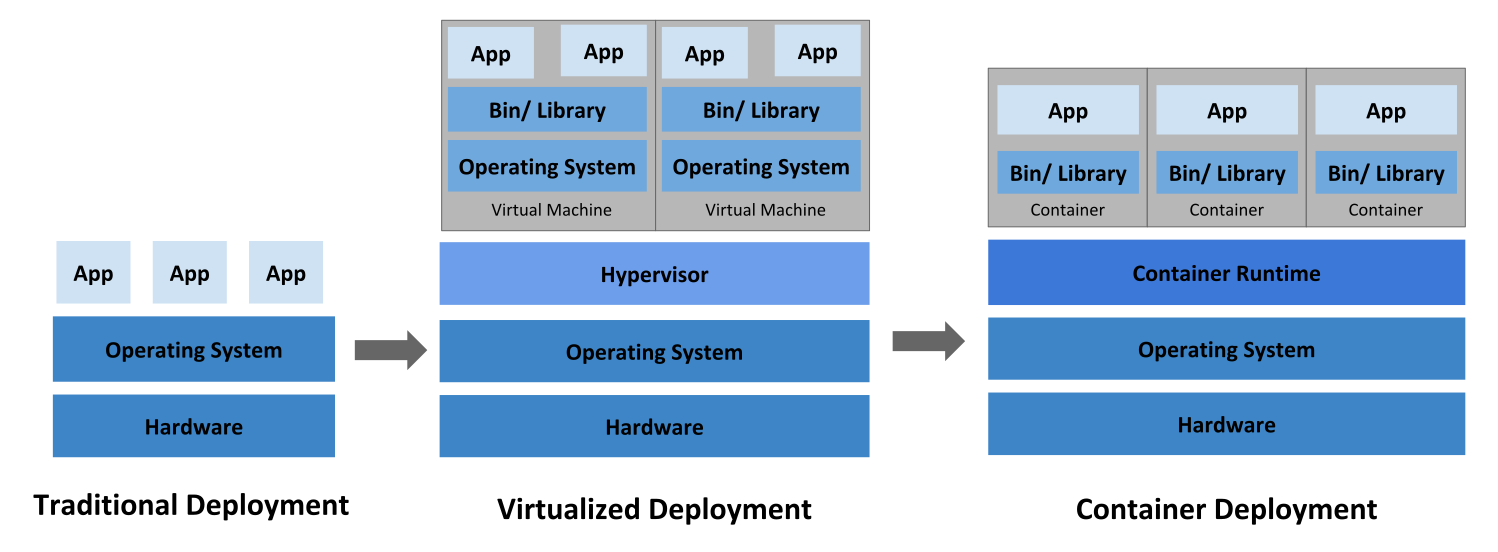
\includegraphics[width=\textwidth]{./../imgs/container_evolution.png}
	\captionsource{Evolution of application deployment.}{\url{https://kubernetes.io/docs/concepts/overview/what-is-kubernetes/}}
	\label{fig:container-evolution}
\end{figure}

Containers can be thought of as lightweight virtual machines. Unlike the
latter, containers share the same kernel with the host machine but still allow
for a very controlled environment to run applications. There are many
benefits to this : separating the development from deployment, portability,
easy resource allocation, breaking large services into smaller micro-services
or support of continuous integration tools (containers greatly facilitate
integration tests).\\

The \textit{Cloud Native Computing Foundation (CNCF)
}\footnote{\url{https://www.cncf.io/}} was founded in the intent of leveraging
the container technology for an overall better web. In a general way, we now
speak of these containerized and modular applications as cloud native computing
:

\textit{``Cloud native technologies empower organizations to build and run
	scalable applications in modern, dynamic environments such as public,
	private, and hybrid clouds. Containers, service meshes, microservices,
	immutable infrastructure, and declarative APIs exemplify this
	approach.}

\textit{These techniques enable loosely coupled systems that
	are resilient, manageable, and observable.  Combined with robust
	automation, they allow engineers to make high-impact changes frequently
	and predictably with minimal toil.``}\footnote{\url{https://github.com/cncf/toc/blob/master/DEFINITION.md}}

Kubernetes\footnote{\url{https://kubernetes.io/}} is the implementation of this
general idea and was announced at the same time as the CNCF. It aims at
automating the administration of a fleet of containers. This system is mostly
description based but still provides a command-line interface to interact with
the resources live. It is industry grade and is now the standard solution for
container orchestration.

\subsection{HPC and Kubernetes}

In this work we use Kubernetes schedulers as batch schedulers because Ryax
makes use of workflow workloads which are closer to batch workloads than
service based workloads. Also, batch scheduling is our domain of origin (Batsim
	was developed in close relation with the teams behind the grid
computing simulator SimGrid \cite{casanova:hal-01017319} and the resource
manager OAR\footnote{\url{http://oar.imag.fr/start}}), and because it is convenient for us to test our
approach with HPC workloads.  However, even though Kubernetes does have means
to handle such workloads like batch
schedulers\footnote{\url{https://github.com/kubernetes-sigs/kube-batch}} and a
special type of
resource\footnote{\url{https://kubernetes.io/docs/concepts/workloads/controllers/job/}},
these two fields differ fundamentally because of the nature of the issues they
tackle. We do not intend to evaluate scheduler performance but rather prove
that such studies are possible with Batsim, which is why this work is conducted
this way. Still, there are perspectives for Kubernetes in the HPC community and
we believe HPC systems could benefit from this work.

The difference between HPC and cloud computing lies in the workloads they are
intended to tackle.  Kubernetes was designed to run applications. Services or
micro services are run in containers and are expected to be available at all
times : they are replicated as many times as desired and restarted whenever a
failure occurs. High availability is at the core of Kubernetes container
management.  On the other hand, depending on implemented scheduling policies,
HPC is focused on metrics such as user wait time, resource usage or energy
cost. One example of a fundamental difference between cluster computing and
batch scheduling is the handling of a task failure. In HPC it is sometimes not
sufficient to restart the single job that failed and the entire submission must
be re-run if it is part of several jobs computed in parallel. In cluster
computing the task is simply restarted without any other consideration -- other
than ensuring its dependencies are restarted with it.

Kubernetes is now the standard for AI and Machine Learning as shown by the many
efforts at making this coupling an efficient environment (\cite{lee2017design},
\cite{233001}, \cite{10.1145/3154842.3154845}), which brought an increasing
interest for container driven HPC aswell and Kubernetes for HPC in particular.
Batch schedulers such as
kube-batch have
been implemented for kube, and numerous HPC applications like
SLURM\footnote{\url{https://slurm.schedmd.com/containers.html}} now support
containers as well.

Indeed, containers have many advantages from which HPC users could benefit
from.
\begin{itemize}
	\item First off, research has shown that Kuberenetes offer similar
		performance to more standard bare metal HPC \cite{8950981}.
	\item Users will get the same environment everywhere making up for a
		uniform and standardized workplace.
	\item Portability : users could seamlessly hop from one infrastructure
		to another based on their needs and criteria like price,
		performance, and capabilities rather than compatibility.
	\item Encapsulation : HPC applications often rely on complex
		dependencies that can be easily concealed into containers.
\end{itemize}
%\begin{figure}[h]
%	\centering
%	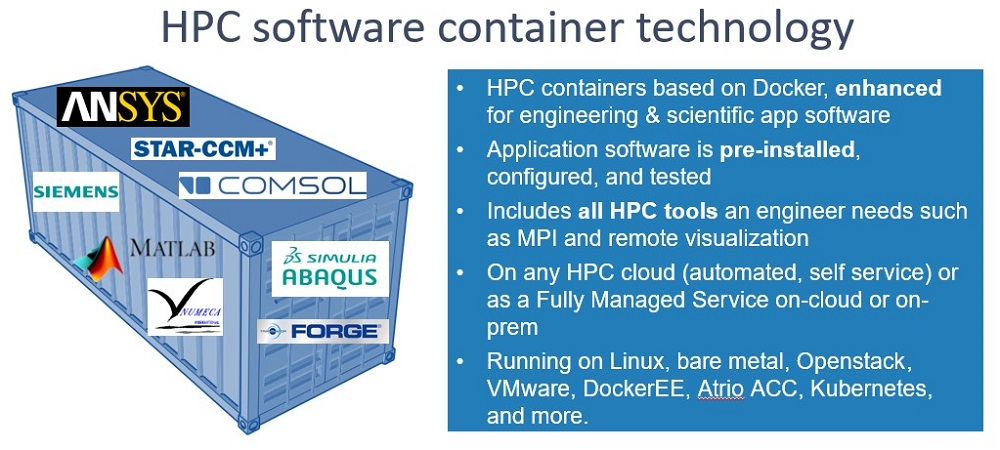
\includegraphics[scale=0.5]{./../imgs/hpc-container.jpg}
%	\captionsource{The container technology for HPC}{https://www.hpcwire.com/2019/09/19/kubernetes-containers-and-hpc/}
%	\label{fig:hpc-container}
%\end{figure}

Despite all those advantages, Kubernetes is not ready yet to be used in proper
HPC environment because it lacks vital components like a proper batch job
queuing system and support for MPI applications. Also, containers are not a
good fit for HPC because most of the isolation given by containers has to be
bypassed \cite{mercier:tel-02284996}. Still, containers are becoming more and
more integrated in modern infrastructures.

\section{Related work}

Not many projects exist on Kubernetes simulation or have been disclosed. We
were able to find two projects that propose simulations of Kubernetes clusters.

JoySim \cite{joysim} is a fully fledged Kubernetes simulator developed in an
industrial context. Simulations are based on synthetic events and their mock
nodes simply simulate a resource usage. The strength of this simulator is its
scalability which it obtains thanks to its very light weight simulated nodes.
JoySim is aimed at studying the quality of the scheduling and its performance
in complex scenarios by generating metrics such as resource usage and
scheduling time. Although, to the best of our knowledge, it is not suited for
batch scheduling and tackles more classic issues for Kubernetes such as
services availability and resource utilization.  The user may specify events to
occur during the simulation in order to test out different scenarios.
Unfortunately, while an open source released in planned, this piece of software
is currently closed source.

k8s-cluster-simulator \cite{k8s-cluster-simulator} is an open source cluster
simulator for evaluating schedulers, which originated from a end of studies
project like this work. Like JoySim, it relies on simple models: pods are
submitted with certain resource requirements, for a certain amount of time. One
can provide any scheduler implementation they want as long as they do so
through their Go interface. This reduces the amount of schedulers that can be
tested to Go implementations only, unless the user is willing to
implement an adaptive layer to support other schedulers.\\

Two simulators are very close to Batsim in terms of capabilities and
objectives, that is to say the study on scheduling policies.

Alea2 \cite{alea2} is a grid computer system simulator based on GridSim. It is
therefore written in Java and cross platform. Like Batsim, its
\textit{ready-to-use} philosophy allow experimenting with different scheduling
policies with little set up overhead.  Alea2 strength lies in its modularity:
its object oriented paradigms make it very easily extensible and customizable.
Unlike Batsim it does not offer a decoupling of the simulator and the decision
process and therefore the user will have to rely on the implemented scheduling
algorithms, although these algorithms cover the most standardly used scheduling
policies.  The user will have to implement other policies he would like to test
out. The simulator handles inputs in the form of \textit{Standard Workloads
Format (SWF)} or \textit{Grid Workloads Format (GWF)}. Batsim proposes a script
to process SWF files into its own input format but does not handle them
directly.

Accasim \cite{10.1007/978-3-319-73353-1_12} is a simulator for studying
\textit{Workload Management Systems (WMS)} in HPC infrastructure. It is similar
to Alea in the sense that the decision process is not decoupled from the
simulator and standard scheduling algorithms are implemented in Accasim, so
that the user does not need to set up extra software in order to start
experimenting. In addition, the user may provide extra data about the system
status (power consumption, temperature or resource failures) in order to
support advanced scheduling algorithms.  These take the form of additional
events transmitted to the simulator. Accasim loads jobs incrementally and
cleans them upon completion which reduces its memory usage compared to Batsim,
which loads everything in memory at the start of the simulation.

What truly distinguishes Batsim from these simulators is the strong decoupling
between the RJMS and the simulator, which allows us to experiment with RJMS
software rather than only studying scheduling policies. This allows us to
evaluate the scheduler computing needs or memory usage independently, as if it
was running in real conditions. Performance wise, we cannot really compare
Batsim with Alea and Accasim because of the fundamental differences in their
models. When Alea and Accasim chose to implement simple models in order to
focus on scalability, SimGrid models, which are consequently Batsim models, are
more advanced and require more computing power.



\chapter{Integrating the simulator into Kubernetes}

\subsubsection{Problematic}

Batsim is able to run simulations of any distributed system, to study any
event-based scheduler that would implement its message protocol. Kubernetes is
a piece of software where all its component, including the scheduler, revolve
around a central API. Everything is then asynchronous as the API can be
accessed anytime by any component.

The question that arises is, can we adapt Batsim to make it support Kubernetes
schedulers? Is it possible to implement an adaptive layer between a synchronous
event based simulator like Batsim and a scheduler implemented following the
asynchronous paradigms of APIs?

It will follow that in order to do so, we re-implemented an API following
Kubernetes specifications and intercepted the scheduler's time to
synchronize it with the simulation time. This allows us to run lengthy
workloads in seconds using a scheduler otherwise supposed to rely on ``real''
machine time. We first describe some technical concepts about Kubernetes and
Batsim, and then describe how we re-implemented the API, intercepted the time,
and handled the synchronization of the different times between Batsim and the
scheduler.


\subsubsection{Batkube features}

TODO: Clearly state what Batkube is capable of, and what it does not do. This
helps describing only the parts of the tools we use while leaving the rest for
the reader to look for on official documentation.

\section{Batsim concepts}

A Batsim simulation is divided into two processes: Batsim itself and the
decision process (the scheduler). Both process exchange via the ZeroMQ
request-reply
pattern\footnote{\url{http://zguide.zeromq.org/page:all\#Ask-and-Ye-Shall-Receive}}.
As a consequence, the scheduler must be event based and implement Batsim's
Protocol.

\begin{figure}[H]
	\centering
	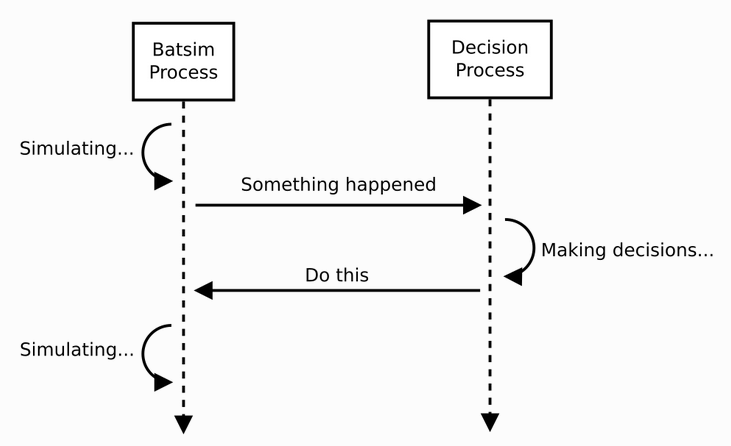
\includegraphics[scale=0.5]{imgs/batsim-sequence-diag.png}
	\captionsource{Exchanges between Batsim and the scheduler}{https://batsim.readthedocs.io/en/latest/protocol.html}
	\label{fig:bati-seq-diag}
\end{figure}

A Batsim platform is a SimGrid platform, defined in the xml format. A node can
endorse the role of \textit{master}, \textit{compute\_resource} or
\textit{storage}. Here we only consider master nodes which host the decision
process, and compute resources to which we add our custom resource capacities.
These additional fields are \textit{core}\footnote{The core field is already
present in the resource definition, but it is not forwarded to Batsim for
unknown reasons at the time this report is written.} which is the amount of cpu
the node has and \textit{memory} which is memory capacity of the node. Of
course, storage resources can be taken into account in future development of
Batkube. Also, we do not consider the links between the nodes for now because
we do not support parallel jobs. Finally, Batsim proposes an energy model that
we decided to ignore as well.\\

Batsim takes one or several workload as inputs, which are json files containing
jobs definitions. The jobs are defined with the following inputs.  First, they
are identified by an \textit{id} which is unique within each workload and are
submitted at a time defined by the \textit{subtime} field. The \textit{res}
field states the number of resources each job requires, although we don't use
this field because we can't specify \textit{which} resource we require. Instead
we pass resource requests as optional parameters. We support the additional
fields \textit{cpu} which has a minimum value of 100m cpu just like Kubernetes
cpu
requests\footnote{https://kubernetes.io/docs/concepts/configuration/manage-resources-containers/}
and \textit{memory} which also complies with Kubernetes compute resource
definitions.  Jobs follow a certain \textit{profile} that defines the nature of
the job.  These profile may be as simplistic as \textit{delay} profile which
makes the resource wait for a given amount of time, or describe parallel tasks
using matrices to describe the amount of exchanges between the allocated nodes.
For now we only consider delays to simplify the implementation of the
simulator. Also, because Kubernetes allows the use of multiple
schedulers\footnote{https://kubernetes.io/docs/tasks/extend-kubernetes/configure-multiple-schedulers/},
we support the field \textit{scheduler} which contains the name of the
scheduler the job should be scheduled with.\\

\begin{figure}
	\begin{minted}{js}
{
    "nb_res": 1,
    "jobs": [
	{"id":"1", "subtime":0, "res": 1, "profile": "delay10"},
	{"id":"2", "subtime":3.4, "res": 1, "profile": "delay10"}
    ],
    "profiles": {
	"delay10": {
	    "type": "delay",
	    "delay": 10,
	    "scheduler": "default",
	    "cpu": "1.5",
	    "memory": "500Mi"
	}
    }
}
	\end{minted}
	\caption{Example of a Batsim workload}
	\label{fig:bat_wl_ex}
\end{figure}

Batsim messaging interface is based on its protocol. Each message is composed
of the field \textit{timestamp} which contains the current simulation time, as
well the field \textit{events} which is a list of events either from Batsim to
the scheduler, or from the scheduler to Batsim. Figure \ref{fig:batmsg_ex}
depicts a standard message sent from the scheduler to Batsim.

\begin{figure}
	\begin{minted}{js}
{
  "now": 1024.24,
  "events": [
    {
      "timestamp": 1000,
      "type": "EXECUTE_JOB",
      "data": {
        "job_id": "workload!job_1234",
        "alloc": "1 2 4-8",
      }
    },
    {
      "timestamp": 1012,
      "type": "EXECUTE_JOB",
      "data": {
        "job_id": "workload!job_1235",
        "alloc": "12-100",
      }
    }
  ]
}
\end{minted}
\caption{Example of a Batsim message}
\label{fig:batmsg_ex}
\end{figure}

Batkube's features are limited because we focused on building a working proof
of concept rather than a fully fledged Kubernetes simulator. This is why only
consider a subset of these messages that we present here. More information on
Batsim's protocol is available on Batsim
documentation\footnote{https://batsim.readthedocs.io/en/latest/protocol.html}

\subsubsection{From Batsim to the scheduler}

\paragraph{SIMULATION\_BEGINS}
contains mostly information about the available resources in the cluster, with
Batsim's configuration.

\paragraph{SIMULATION\_ENDS}
is sent at the very end of the simulation: all jobs have finished, and no more
jobs are left in the queues. Batsim exits on this message.

\paragraph{JOB\_SUBMITTED}
notifies the scheduler that a new job has been submitted. It contains
information about the job type, id and specifications. We only consider jobs of
type \textit{delay} to simplify the models. Delay jobs specifications boil down
to the delay length, to which we add resource requests.

\paragraph{JOB\_COMPLETED}
notifies the scheduler that a job has ended, specifying the reason for it. We
only consider situations where all jobs complete correctly. Their state is then
always COMPLETED\_SUCCESSFULLY in our case.

\paragraph{REQUESTED\_CALL}
is an awnser to a CALL\_ME\_LATER event sent by the scheduler.

\subsubsection{From the scheduler to Batsim}

\paragraph{CALL\_ME\_LATER}
is an incentive from the scheduler for Batsim to wake up at a certain
timestamp. When the timestamp is reached in the simulation, Batsim will send a
REQUESTED\_CALL to the scheduler. In our case, this particular exchange will
serve as the base for time synchronisation between the scheduler and Batsim.

\paragraph{EXECUTE\_JOB}
is sent when the scheduler has made a decision. It contains the id of the job
at stake and the id of the resources it has been scheduled to.

\subsubsection{Bidirectional}

\paragraph{NOTIFY}
is used to send some information to the other peer. In our case, we use the
NOTIFY containing no\_more\_static\_job\_to\_submit to determine if the
simulation has ended: knowing that there are no more jobs susceptible to be
scheduled allow us to fast forward to the end of the simulation, thus saving
execution time.\\

Batsim's output takes the form of a csv file containg information about the
jobs executions. Mainly we take interest in their submission time, execution
time and waiting time. Again, a detailed list of Batsim outputs can be found on
the
documentation\footnote{https://batsim.readthedocs.io/en/latest/output-jobs.html}.
During our experimentations with Batkube we interest ourselves in two metrics
that can be computed from this output:
\begin{itemize}
	\item The \textit{makespan}, which is the total length of the
		simulation. It is defined as the timestamp at which the last
		job finishes executing, minus the origin (in this case, zero).
	\item The \textit{mean\_waiting\_time}, which is the mean time the jobs
		spent waiting for a scheduling decision. The waiting time is
		defined by the duration between the submission time and the
		starting time (here the starting time is equivalent to the time
		at which the job was scheduled. We will see later that these
		two times do not correspond in Kubernetes.)
\end{itemize}

\section{Kubernetes concepts}

Kubernetes is now a large ecosystem to which more than 2 700 developers have
contributed over the years. In this section we present the fundamental concepts
and the components that make up Kubernetes.

\begin{figure}[h]
	\centering
	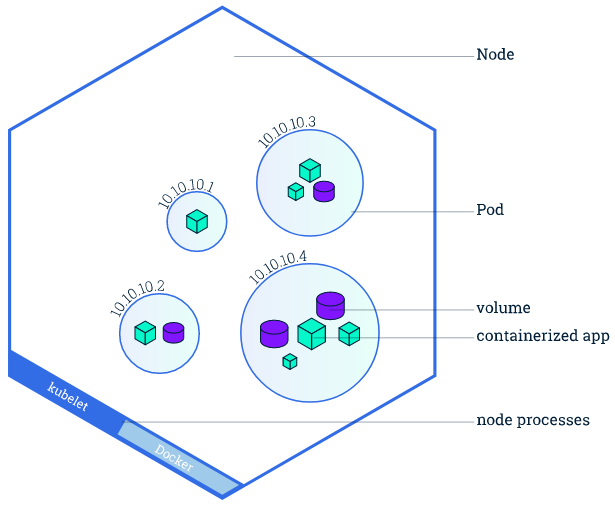
\includegraphics[scale=0.5]{./imgs/node-overview.png}
	\captionsource{Node overview}{https://kubernetes.io/docs/tutorials/kubernetes-basics/explore/explore-intro/}
	\label{fig:node-overview}
\end{figure}

The basic processing unit of Kubernetes is called a \textbf{pod} which is
composed of one or several containers and volumes\footnote{Because of their
	transient nature, containers can not store data on their own. A volume
	is some storage space on the host machine that can be linked to
containers, in order for them to read and write persistent information.}. The
type of application they contain vary depending on the context: in a web
platform context a pod most often hosts a service or micro-service that must be
available at all times, in opposition to a batch processing context where it
runs an application that is to be executed in a finite amount of time.  Pods
are bundled together in \textbf{nodes} (figure \ref{fig:node-overview}) which
are either physical or virtual machines. They represent another barrier to pass
through to access the outside world which bundles pods under the same network
to facilitate communication between them, and enables the use of proxies to
access the underlying services. A set of nodes is called a \textbf{cluster}
which is the highest abstraction layer in Kubernetes.

Nodes take the idea of containerization further than plain containers by
encapsulating the already encapsulated services.  Each node runs at least one
pod, the \textbf{kubelet}, which is a process responsible for communicating
with the rest of Kubernetes. More precisely, the kubelet communicates with the
\textbf{kube-api-server} which is responsible for the whole cluster. We refer
to this API as the api-server, as it is called within the Kubernetes community.
This API server, as well as the other components of the \textbf{Control Plane}
(figure \ref{fig:kube-components}), can be run on any machine but for
simplicity they are set up on the same machine at start up. This machine is
often called the \textbf{master} node and typically does not run any other
container.

As stated before Kubernetes revolves around its API server which is its central
component. All operations between components go through this REST API. These
operations take various forms like user interactions through the commande line
interface \textbf{kubectl}, scheduling operations or management of cluster data
on \textbf{etcd}. We then decided to re-build the API in order to simulate any
cluster to -- almost -- any Kubernetes scheduler.

TODO: Talk about Kubernetes schedulers. What they are based on, how they communicate to Kubernetes.

\begin{figure}[h]
	\centering
	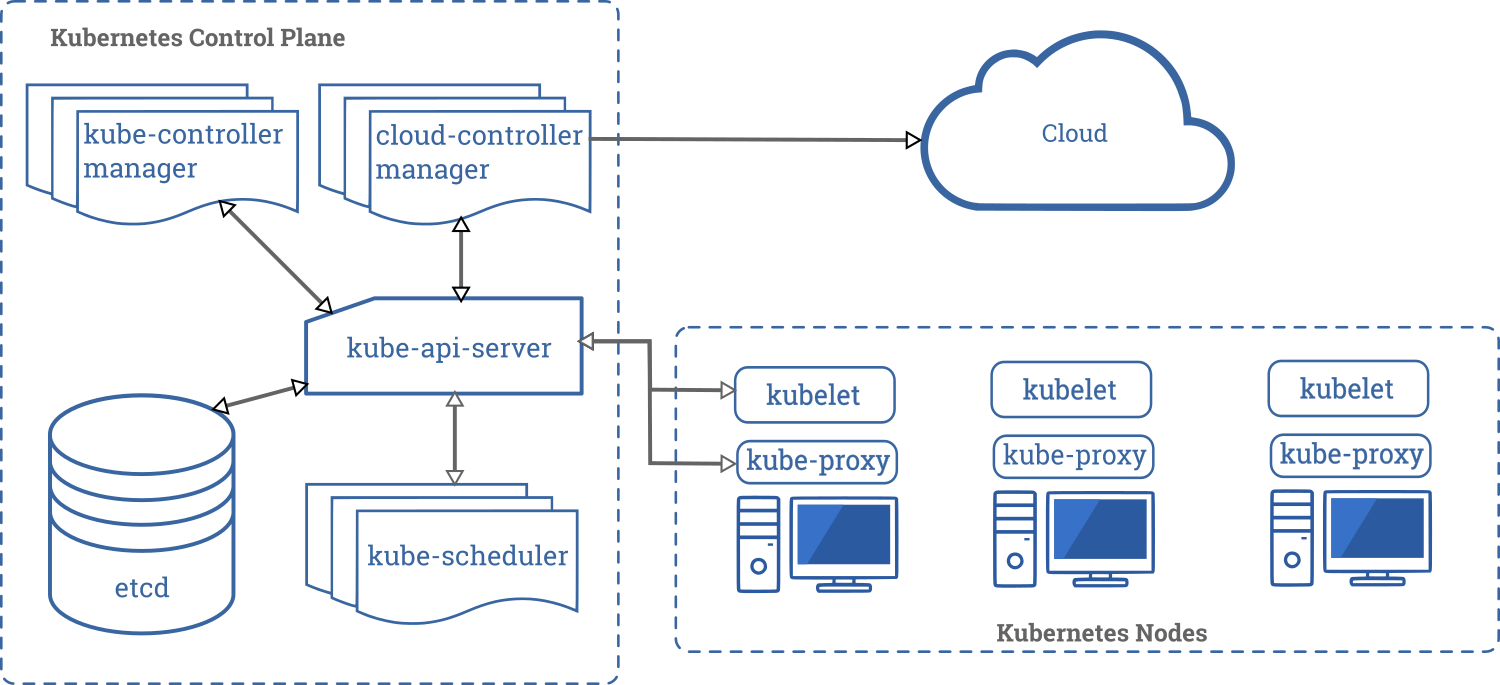
\includegraphics[width=\textwidth]{./imgs/components-of-kubernetes.png}
	\captionsource{Components of Kubernetes}{https://kubernetes.io/docs/concepts/overview/components/}
	\label{fig:kube-components}
\end{figure}

\section{General architecture of Batkube and its integration with Kubernetes and Batsim}

\subsection{Integration with Kubernetes}

In order to adapt Kubernetes schedulers for use with Batsim we need to position
ourselves between the Kubernetes scheduler and the cluster. There are several
options here, at different levels of the cluster. All these are made possible
by the fact that Kubernetes is entirely open source and can be reverse
engineered and modified to suit our needs. First we present the options we
considered but did not choose, and then we explain how we wrote a custom REST
API which acts as a Kubernetes cluster to the scheduler, and as an event based
scheduler to Batsim.

\subsubsection{In between the api and the kubelets}

This is the lowest level option. We position the simulator so as to simulate
just the infrastructure and avoid tampering with Kubernetes resource
management, which is done in their API. This approach would allow us to
effortlessly use any Kubernetes scheduler once their API is supported by
Batkube, and potentially produce the most accurate results. However,
interactions between the kubelets and the API are not documented because the
typical user is not supposed to have to deal with this part of Kubernetes. This
would hinder the development of Batkube because a reverse engineering process
would be required beforehand to understand the intricacies of internal
Kuberenetes exchanges.

\begin{figure}[h]
	\centering
	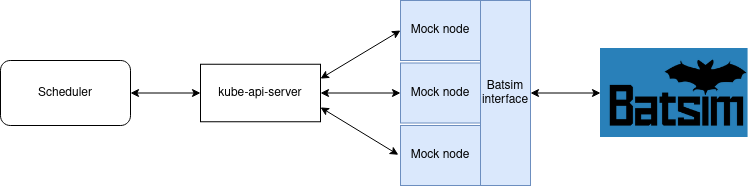
\includegraphics[width=\textwidth]{imgs/architecture-as-kubelets.png}
	\caption{Mocking the cluster itself.}
	\label{fig:mock_nodes}
\end{figure}

\subsubsection{Custom client-go}

Most Kubernetes schedulers rely on
client-go\footnote{https://github.com/kubernetes/client-go}, which is a Go
client for the api-server. It is a library implementing various tools to help
schedulers converse with the API. By altering this client and patching
schedulers so they use our client instead, we can make it exchange with Batsim
instead of the API. 

\begin{figure}[h]
	\centering
	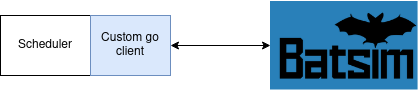
\includegraphics[scale=0.8]{imgs/custom-go-client.png}
	\caption{Custom Go client to redirect scheduler communications to Batsim}
	\label{fig:custom-go-client}
\end{figure}

Contrary to the kubelets, client-go is a user interface and therefore it is
documented, facilitating reverse engineering of its source code. Still, it
represents thousands of lines of code and altering it to our needs would not be
an easy feat.  The other drawback to this approach is that Batkube would only
support schedulers written in Go and making use of client-go, although this
should not be an issue as the only kubernetes scheduler we could find that does
not rely on client-go is a toy scheduler written in bash \cite{bash-scheduler}.

\subsubsection{Custom API}


Re-implementing the API offers a middle ground between the low level and
undocumented solution of the mock nodes, and the higher level and technically
challenging solution of a client-go fork. Again, there are several options here.

A partial reimplementation of the API would save us the task of building a new
API from the ground up. However this would imply digging deep into the
api-server code in order to understand how the api is organized and what code
we would have to alter. In the end, it is easier to simply build a new API,
since there are tools to help us generate it from its specification.

\begin{figure}[h]
	\centering
	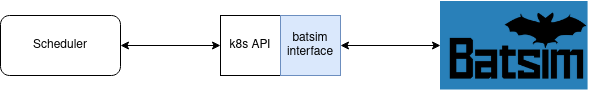
\includegraphics[scale=0.8]{imgs/partial-reimplem.png}
	\caption{Partial reimplementation of the api-server.}
	\label{fig:partial_reimp}
\end{figure}

Furthermore, building a new API allows us to consider only the endpoints we
need and have complete control over the source code. The technically
challenging aspect here is Kubernetes resource management. Indeed, we need to
provide the scheduler with expected informations about the cluster state if we
want to obtain a correct behavior from it, and while the endpoints of the API
are well documented, Kubernetes team did not write lengths about how resources
are managed internally.

\begin{figure}[h]
	\centering
	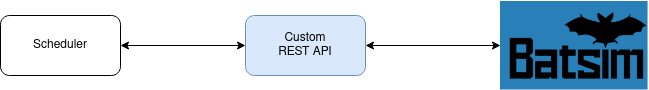
\includegraphics[width=\textwidth]{imgs/custom-restapi.png}
	\caption{Custom REST API in between the scheduler and Batsim.}
	\label{fig:custom-api}
\end{figure}

\subsection{Architecture of Batkube}

Figure \ref{fig:batkube-architecture} depicts the architecture of Batkube,
which is written in Go.  The central component is the \textbf{broker}. It
handles the messages coming from Batsim and the scheduler while ensuring time
synchronization between them. It is responsible for translating and forwarding
messages between Batsim and the scheduler and orchestrates the synchronization
between the two parties.  \textbf{batsky-go} intercepts the calls to Go
\textit{time} library to ensure the scheduler's time is based on the simulation
time instead of machine time. Time requests are forwarded to Batkube which
replies with the current simulation time.  The complete process to ``hijack''
scheduler time is explained in section \ref{sec:time-hijack}. The \textbf{rest
api} is the reimplementation of the Kubernetes api-server. It ensures the
scheduler gets all the necessary information on the cluster state to make its
scheduling decisions, and it is also the receiver of those decisions. Section
\ref{sec:api} explains how we built this API and a tool to automatically
generate its code from the api-server specification.  \textbf{translate} is a
utility package providing functions to translate Kubernetes resources to Batsim
messages, and \textit{vice versa}.

\begin{figure}[h]
	\centering
	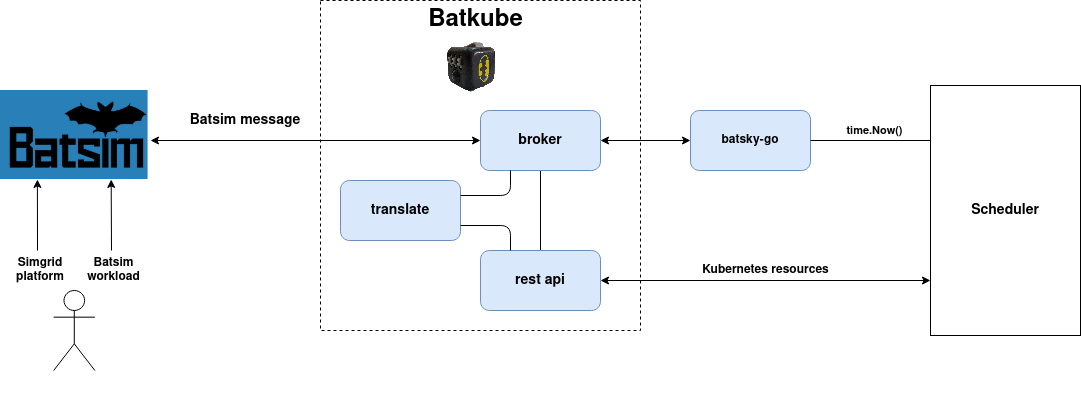
\includegraphics[width=\textwidth]{imgs/batkube-architecture-3-synchro.png}
	\caption{Architecture of Batkube}
	\label{fig:batkube-architecture}
\end{figure}

\section{Building the API} \label{sec:api}

The API of Kubernetes follows the
OpenAPI\footnote{https://www.openapis.org/about} 2 specification which is a
standard for describing APIs. Luckily tools exist to generate such
specification from source code, but also to generate code from a specification.
Since the Kubernetes API specification is available on their
reposotory\footnote{https://github.com/kubernetes/kubernetes/blob/release-1.18/api/openapi-spec/swagger.json},
we were able to use such tools. This allowed us not to implement boiler plate
code by hand and fill the gaps where they needed to be filled, leaving empty
the endpoints we do not need. These endpoints can be dealt with later for
future development of the simulator. For this project we used
go-swagger\footnote{https://github.com/go-swagger/go-swagger/tree/master/examples/stream-server}
to generate our code and the API specification corresponds to the release 1.18
of Kubernetes. One downside of this method is that go-swagger forbids to tamper
with the code of the server itself, although we did not need to during this
project.\\

In order to enable communication between Batsim and the scheduler we need to
translate Batsim messages into Kubernetes resources that can be retrieved by
the scheduler and scheduler decisions to Batsim messages. Batsim Jobs are
simply translated to pods. Jobs do exist in Kubernetes, but they are simply
wrappers around pods: when submitting a job to the (real) api-server, the api
ensures that a pod is created and executed to completion. In our case, we do
not need such intermediate. Compute resources are simply translated to
Kubernetes nodes.

\section{Time interception} \label{sec:time-hijack}

Kubernetes schedulers are not event based schedulers. They constantly check on
the cluster state and make decisions accordingly, therefore they are based on
machine time to make their decisions. However, in order to have correct
simulations, the scheduler needs to be synchronized with simulation time. We
then need to intercept all calls to machine time to redirect them to the
simulator. There are two approaches to this: either we patch the C library used
by Go (figure \ref{fig:patch-C}) and compile Go using our library, or we patch
Go's time library (\ref{fig:patch-Go}) and then patch the scheduler so it uses
our library instead of the official one.

\begin{figure}[]
	\begin{subfigure}{0.5\textwidth}
		\centering
		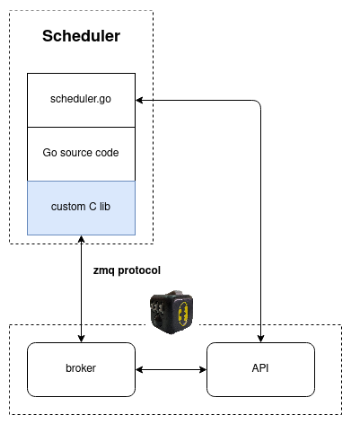
\includegraphics[scale=0.8]{imgs/time-hijack-C.png}
		\caption{Option A: patching the C library}
		\label{fig:patch-C}
	\end{subfigure}
	\begin{subfigure}{0.5\textwidth}
		\centering
		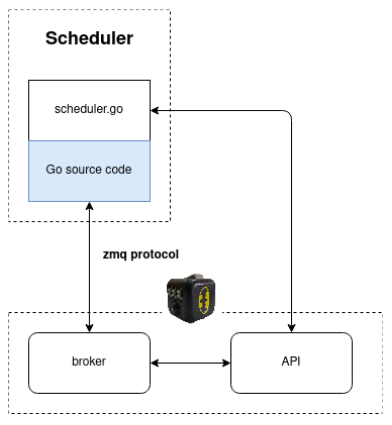
\includegraphics[scale=0.75]{imgs/time-hijack-Go.png}
		\caption{Option B: patching Go}
		\label{fig:patch-go}
	\end{subfigure}
	\caption{Different approaches to intercept the scheduler calls to machine time}
	\label{fig:patch-time}
\end{figure}

An attempt was first made for the custom C library, which is the lowest level
solution. Going for the low level solution would truly redirect all calls to
machine time which is something we can not guarantee with the second option, as
we will see in section \ref{sec:patch-scheds}. This approach proved challenging
due to circular dependency issues and was ultimately abandoned. We opted for
the second option which consist of modifying Go source code, which requires
some additional work to patch the schedulers but was actually easier to
implement.

\subsection{Redirection of time requests to Batkube}

The module in charge of this time redirection is called
\textbf{batsky-go}\footnote{https://github.com/oar-team/batsky-go}, which re
implements \texttt{time.Now()} as well as timers and tickers. Timers are
structures that are instantiated with a duration as input, that notify the
caller once this duration is elapsed. Timers can be reset, modified or deleted
after initialization, which make their implementation tricky in a parallel
computing context. Tickers are essentially the same structures as timers,
except they regularly notify the caller with the given period of time instead
of exiting like timers would.

In order to explain batsky-go algorithms as clearly as possible we need to
provide some context about Go channels, which are structures made for running
code in parallel. Go allows the user to run multi threaded code easily thanks
to its \textbf{go routines}. Whenever in the code the user may create a routine
which will create a new thread and launch the given code parallel to the
encapsulating function. Essentially, this creates a child process -- and
introduces the risk of creating fork
bombs\footnote{https://github.com/aaronryank/fork-bomb/blob/master/fork-bomb.go}.
Go channels are \textit{``a typed conduit through which you can send and receive
values with the channel operator, <-''}\footnote{source:
https://tour.golang.org/concurrency/2}

\begin{figure}[H]
	\begin{minted}{go}
ch <- v    // Send v to channel ch.
v := <-ch  // Receive from ch, and
           // assign value to v.
   \end{minted}
   \caption{Usage of a Go channel}
   \ref{fig:go-channel}
\end{figure}

\SetKwInput{KwInput}{Input}
\SetKwInput{KwOutput}{Output}

\begin{algorithm}[H]
\DontPrintSemicolon
\KwResult{Current simulation time}
\KwInput{d: timer duration, req: requests channel, res: response channel map}
\KwOutput{now : simulation time}

\If{requester loop is not running}{
	go runRequesterLoop() \tcc{There can only be one loop runing at a time}
}
id = newUUID()\;
m = newRequestMessage(d, id) \tcc{Requests are identified using uuids}
resChannel = newChannel()\;
res[id] = resChannel \tcc{A channel is associated with each request}
req $<$- m \tcc{The code blocks here until request is handled}
now = $<$-resChannel \tcc{The code blocks here until response is sent by the requester loop}
return now\;
\caption{Time request (time.now())}
\label{alg:now}
\end{algorithm}

\begin{algorithm}[H]
\DontPrintSemicolon
\KwInput{req: requests channel, res: response channel map}
\While{Batkube is not ready} {
	wait\;
}
requests = []request\;
\While{req is not empty} {
	m = $<$- req \tcc{Non blocking receive}
	requests = append(requests, m)\;
}
sendToBatkube(requests) \tcc{Only requests with duration > 0 are actually sent. Batkube will always anwser.}
now = responseFromBatkube()\;
\For{m in range requests} {
	res[m.id] $<$-now \tcc{The caller continues execution upon reception}
}

\caption{Requester loop}
\label{alg:reqLoop}
\end{algorithm}



\subsection{Patching schedulers} \label{sec:patch-scheds}

TODO: Explain the AST approach and how it is not a plain sed. (conflict in the
resources used, we have to replace all calls to time's \textbf{functions} and
leave the \textbf{objects} as they are).

\section{Time synchronization}

TODO: explanatory text on this diagram. Explain the different parameters:
timeout, max \& base timestep \& backoff multiplier, min delay, scheduler crash
detection, fast forward on no pending jobs.
\begin{figure}[H]
	\centering
	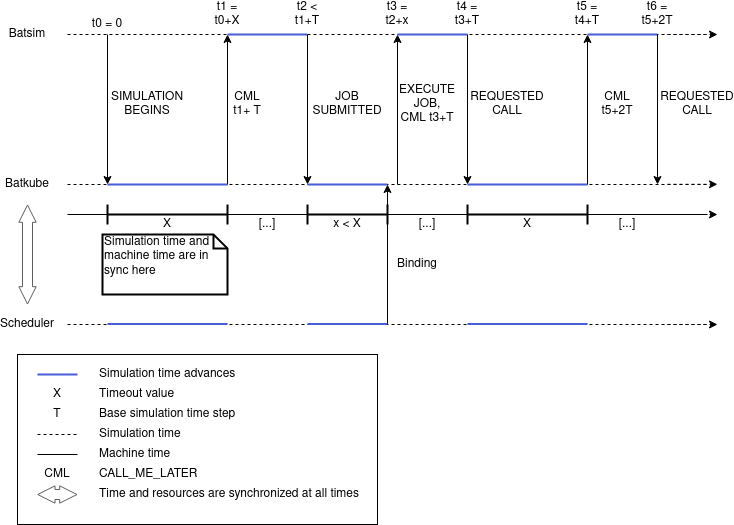
\includegraphics[width=\textwidth]{imgs/lignes_de_temps.png}
	\caption{Time sync between the three components. The broker has to take
	into account both machine time and simulation time.}
	\label{fig:time_sync}
\end{figure}


\chapter{Evaluation and discussion}

Because SimGrid has already been thoroughly tested and validated, we do not
need to run extensive experiments to validate Batkube simulation models.
Moreover, since we only consider simple delay jobs, validation is not really
necessary. Still, even though the underlying models are sound, Batkube adds a
considerable overhead to Batsim because of the time synchronization between the
simulator and the scheduler. We want to verify to what extent time manipulation
impacts the scheduler behavior, and also that Batkube's fake Kubernetes API
mimics the real API well enough to let the scheduler run as expected. We then
conducted some validation experiments with simple workloads to verify that the
scheduler was correctly making its decisions.

In the next sections, we present the workloads and platforms we chose to study,
how we conducted experiments on a real cluster, and a study on Batkube's
parameters and their effect on the outputs.

\section{Experiments environment}

The entirety of the experiments are done with the default Kubernetes scheduler
\textbf{kube-scheduler} release \textbf{v1.19.0.rc-4} (commit 382107e6c84).
This choice was made because it is the standard choice for Kubernetes and
therefore the most commonly used scheduler in the industry, and because
supporting another scheduler would mean more development time which we did not
have. Still, it allowed us to conduct experiments to verify that the scheduler
behavior was not altered by Batkube.  All scripts used to run the experiment,
process the workloads and generate the graphs present in this report -- along
with some results -- are available on
\textit{batkube-test}\footnote{github.com/oar-team/batkube-test} repository.

\subsection{Real experimental testbed}

In order to validate the simulator results we then need to compare it against
workloads run on a real cluster. For reproducibility and simplicity sake, we
choose to validate the simulator with an emulated cluster run in containers. We
use k3s, which is a lightweight version of Kubernetes (k8s). It has all the
essential features of Kubernetes we would need and has become a standard in the
industry whenever administrators do not wish to run fully fledged versions of
Kubernetes.\\

\begin{figure}[H]
	\centering
	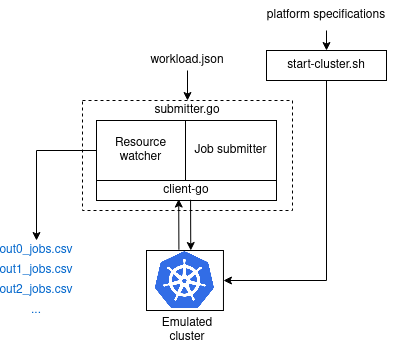
\includegraphics[scale=0.7]{./imgs/prot-k3s.png}
	\caption{An emulated experiment.}
	\label{fig:emulated-expe}
\end{figure}

Figure \ref{fig:emulated-expe} illustrates how this is done. First, we create a
k3s cluster run using docker-compose, which is a tool enabling us to
conveniently create one or several network of containers. Our cluster contains
one master node and several workers which will run our pods. Then, a Go script
which takes a Batsim workload as an input submits the jobs at the right time,
watches the cluster state regularly, and writes the ouputs to csv files --
which have the same format as Batsim's csv output files. We run each workloads
10 times in order to get statistically meaningful results, except for the
realistic workload which we only run once because it is already 10 hours long.

The emulated cluster is limited in terms of variety and capacity. First,
\texttt{start-cluster.sh} only allows the nodes to have the same amount of
available cpu, memory or storage because there was no need for any complex
system for our experiences. Secondly, the maximum amount of cpu, memory or
storage we can make available for each node is capped to the host system
capacities. For example, if the host system possesses 8 cpu cores, the nodes
will have a maximum of 8 cpu available. This will have implications when trying
to run workloads recorded on real systems: either we get to find a workload
that complies with the host system capacity (which is very unlikely), or we
adapt the workload so the jobs requirements do not exceed the host
capabilities (see section \ref{sec:studied-workloads}).

\subsection{Studied workloads} \label{sec:studied-workloads}

We consider three workloads, representing three different situations. The first
two are simplistic and very controlled, and the last one depicts a more
realistic case. In all cases the required resources are only quantified in cpu
only to simplify the study. Note that Batkube does support memory requets, we
just do not wish to add this other layer of complexity to our experiments.

\begin{itemize}
	\item A \textit{burst} workload, consisting in an important amount of
		jobs submitted at once.  200 delays with duration 170s and
		requesting 1 cpu are submitted at the origin.
	\item A \textit{spaced} workload, where jobs of the same nature are
		submitted at regular intervals.  200 delays with duration 170s,
		and requesting 1 cpu are submitted every 10s.
	\item A \textit{realistic} workload, which is a trace extracted from the  Karlsruhe Institue of Technology ForHLR II System.
\end{itemize}

The first two workloads are straight forward and could be generated with the
use of a plain text editor (understand \texttt{vim} and its macros). The third
workload required more processing to be obtained.  

\subsubsection{Standard Workload Format processing}

Batsim provides a tool to translate SWF files to its own json definition. It
also works as a workload preprocessor, although we want to process SWF files
very specifically to suit our needs which is why a custom script was
implemented.

First, a trace in standard workload format (swf) was obtained on a web
archive\footnote{https://www.cs.huji.ac.il/labs/parallel/workload/logs.html}.
The chosen workload was \texttt{KIT-FH2-2016-1.swf} (we give the file name for
the reader to find the workload on the archives) because it is the most recent
and is relatively lightweight. It is composed of 114,355 jobs spanning over 19
months. Secondly, \texttt{evalys}\footnote{https://github.com/oar-team/evalys}
allowed us to extract a subset of this workload lasting for a given period of
time and with a given mean utilization of the resources. We chose a period of
10h with 80\% utilization of the resources so as to keep reasonable experiment
durations -- Later on we experiment with larger workloads to test out Batkube's
limits in terms of scalability.  The third step is translating this extracted
workload to a \texttt{json} file that can be read by Batsim, which is done with
a script written in Go.

After extracting this subset, we are left off with a workload containing jobs
spanning up to 45h and using up to 24048 cpu (or cpu cores), which is undoable
at our scale on our emulated cluster. We need to trim job durations as well as
cpu usage, as we are limited in cpu by the host machine. This is done during
the translation to the \texttt{json} format. The durations are trimmed down to
a maximum of one hour and the cpu usages are normalized so the maximum amount
of cpu requested equals the amount of cpu available per node on the host
machine. Otherwise, the job would not be schedulable which would not present
much interest. We end up with a trace composed of 39 jobs spanning over 10
hours, with a maximum job length of one hour and cpu usage ranging from 0
(excluded) to 5.9 (even though the host machine had 6 cores, Kubernetes
scheduler did not allow for a job to be scheduled on a node it would use 100\%
resources of).

\subsection{Studied platforms}

The platform used for the first two workloads, \textit{burst} and
\textit{spaced} is composed of 16 nodes each heaving one cpu. For the
\textit{realistic} workload however, we use a single node composed of six cores
for the following reasons.

First, the host machines where the experiments were conducted had six cpu cores
available. This means that if we want to be able to run an emulated cluster
equivalent to this platform we can't exceed six cpu per node.  We use the
maximum amount of available cores in order so as not to obtain too low values
when normalizing the resource requests on the jobs. Indeed, Kubernetes only
allows for a precision of 1 milicpu, so any value bellow that is not considered
a significant number. Normalizing on six cpus instead of one allows us to get
more significant number. Also, only one node gives us a satisfactory overall
resource usage: with more than one node one resource is almost always available
making the scheduling operations trivial.

\section{Study of the simulator parameters} \label{sec:params-eval}

The simulator has a few parameters that impact the simulation speed and
accuracy. The objective is to study the effects of these parameters on the
simulation to better understand the scheduler behavior when running in
coordination with Batkube.\\

The objective here is to fine tune the parameters in order to find a compromise
between accuracy and scalability. We want to know which combination lead us to
the most stable results, while keeping simulation time as low as possible.

The parameters are:
\begin{itemize}
	\item The \textit{minimum delay} we have to spend waiting for the
		scheduler.
	\item The \textit{timeout} value when waiting for scheduler decisions.
	\item The \textit{maximum simulation time step}, which is the maximum
		amount of time Batsim is allowed to jump forward in time.
\end{itemize}

We first study these parameters one by one by fixing the other parameters to
some other value, then we study what effects these parameters have in respect
to one another, and finally we conduct scalability experiments to test
Batkube's stability and performances on large workloads.

\subsection{Minimum delay}

Earlier in the development of batkube we noticed that not leaving enough time
to the scheduler each cycle lead it to crashes and deadlocks, ultimately
failing the simulation. This time is independent from any decision making we
would receive from it which is why it is called \textit{minimum wait delay}
instead of a plain \textit{timeout} - which is in fact another parameter we
will study later.

For each workload, we compute the crash rate every 5ms, from 0ms to 50ms. Each
point is made by running the simulation 15 times and recording the exit code as
well as the simulation time. The other parameters are: \texttt{timeout=20ms};
\texttt{max-simulation-timestep=20s}. As we will see later those do not offer
acceptable simulation results but they allow us to run prompt simulations, as
accuracy do not concern us here.\\

\begin{figure}
	\centering
	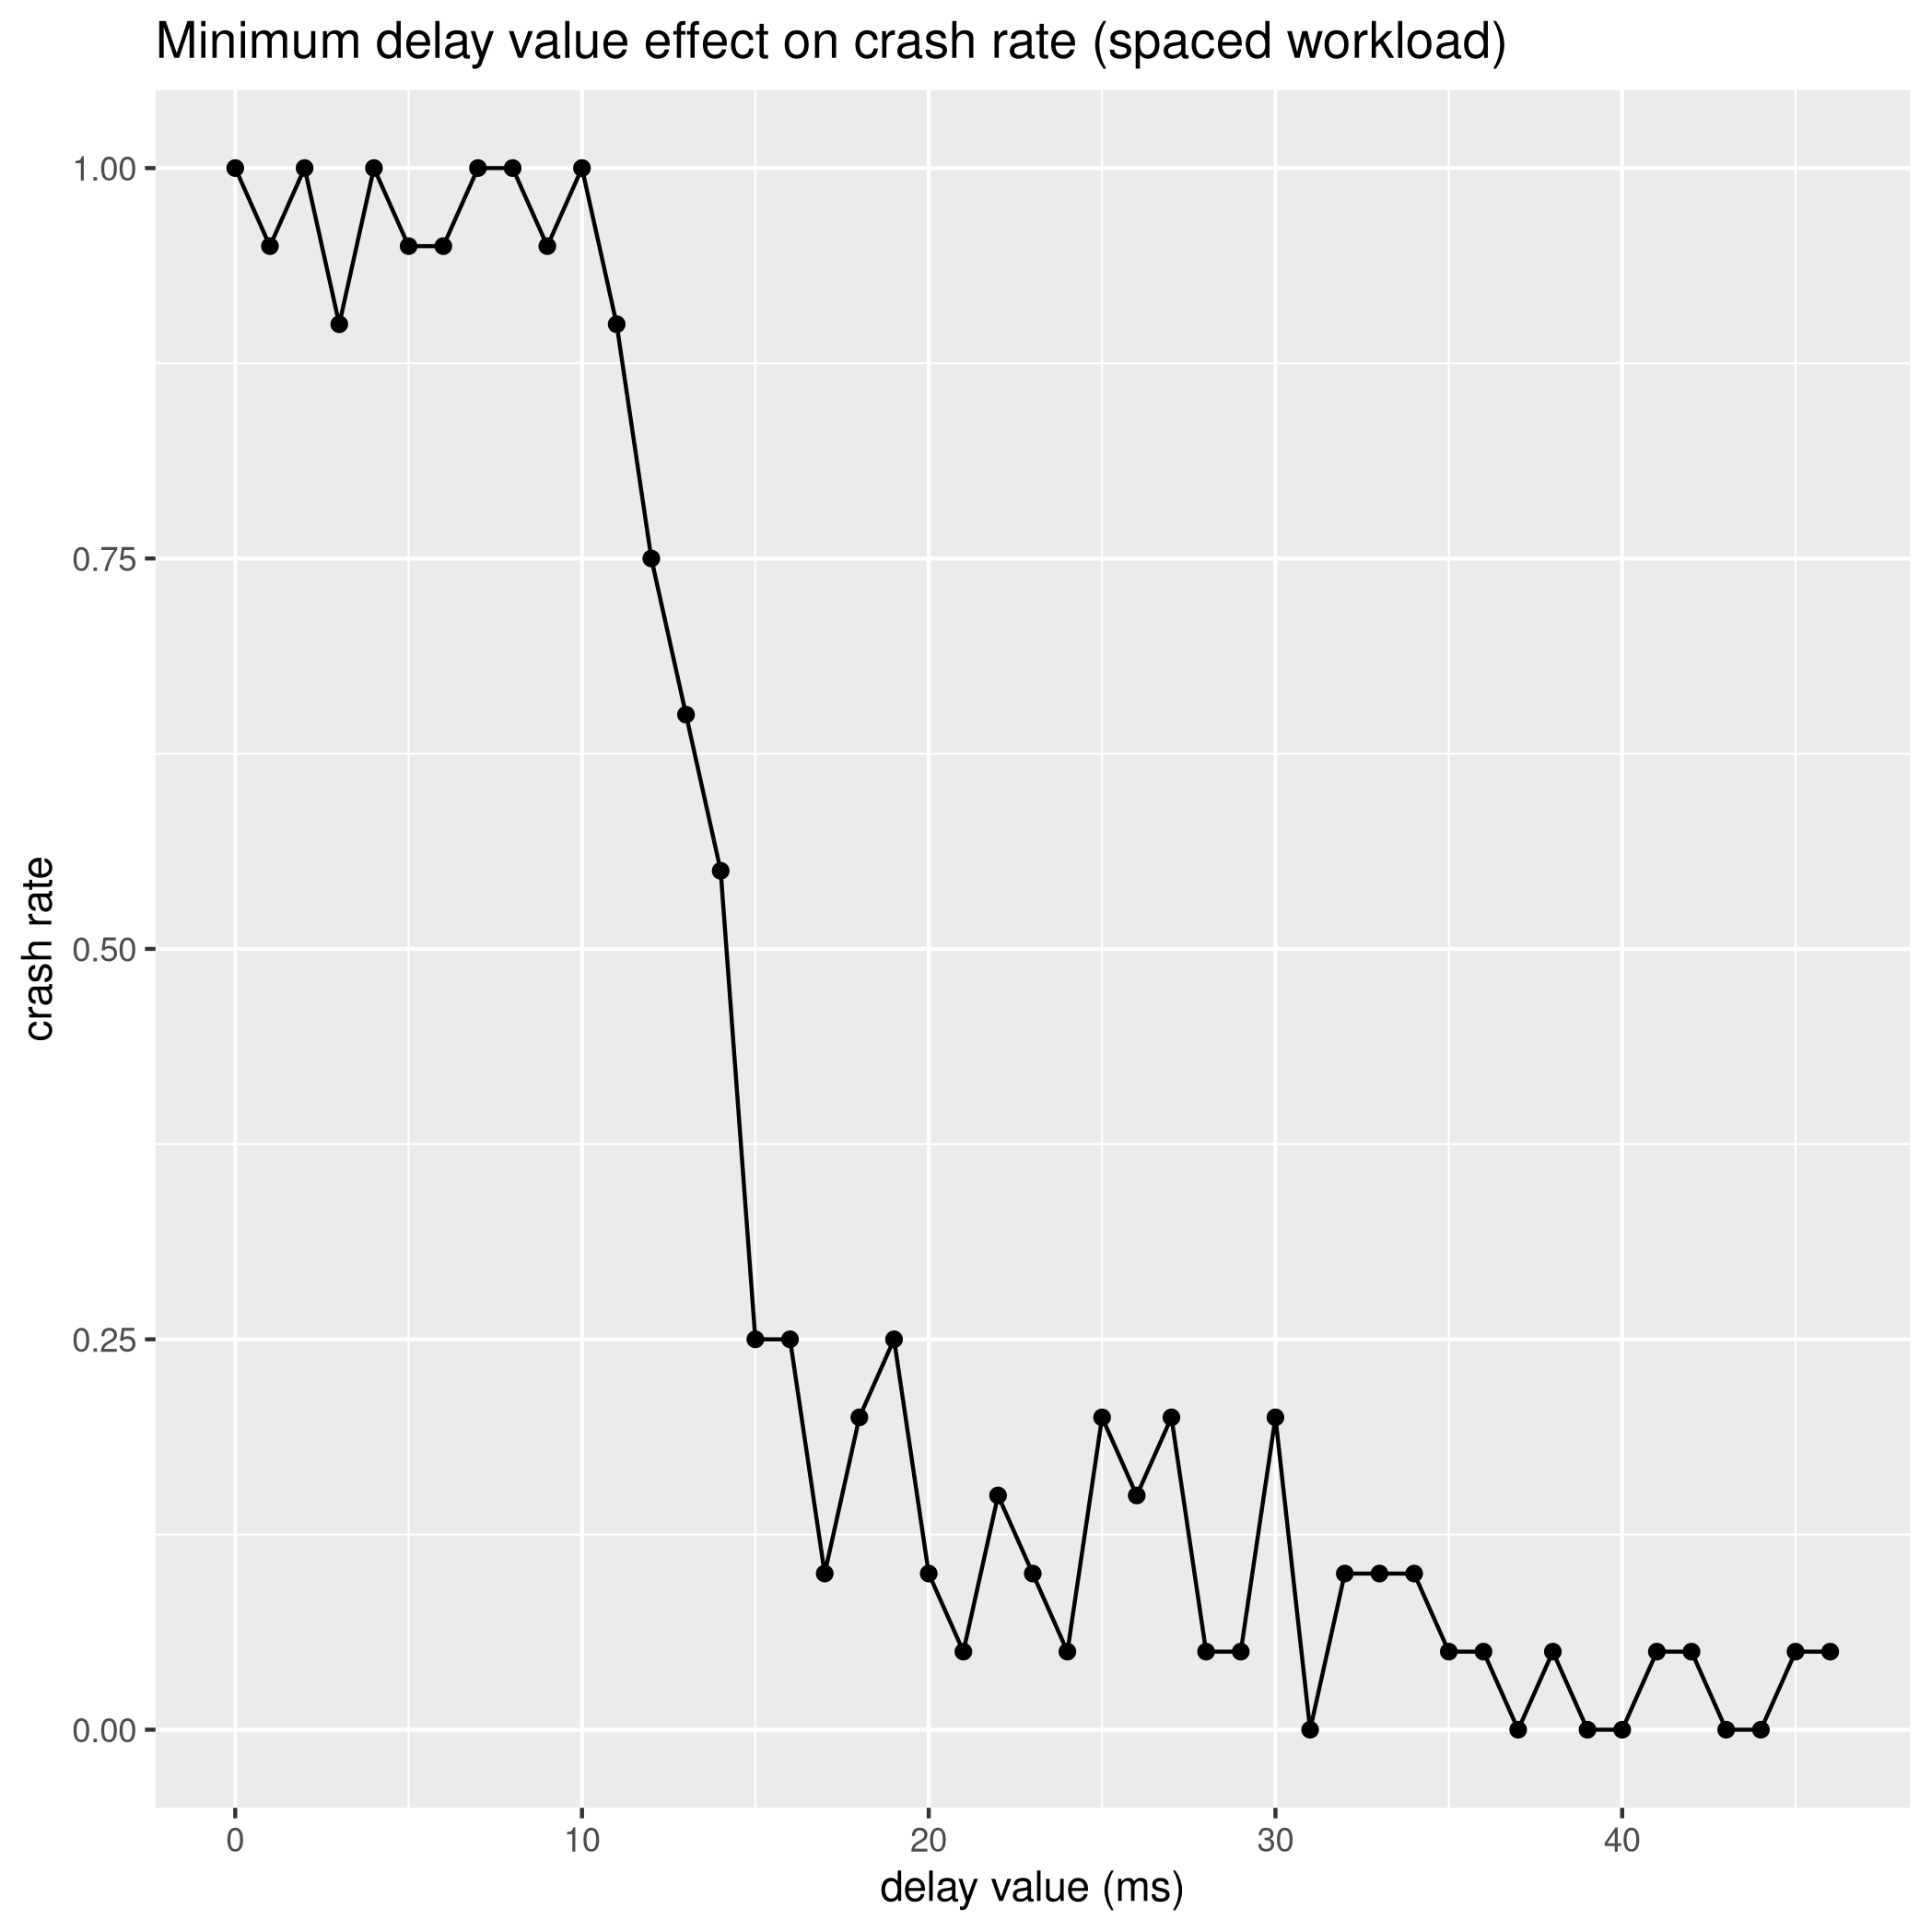
\includegraphics[width=0.45\textwidth]{imgs/min-delay_spaced_200_delay170_crash_old.png}
	\caption{Crash rate of the simulations against minimum delay.}
	\label{fig:min-delay_crash}
\end{figure}

\begin{figure}
	\centering
	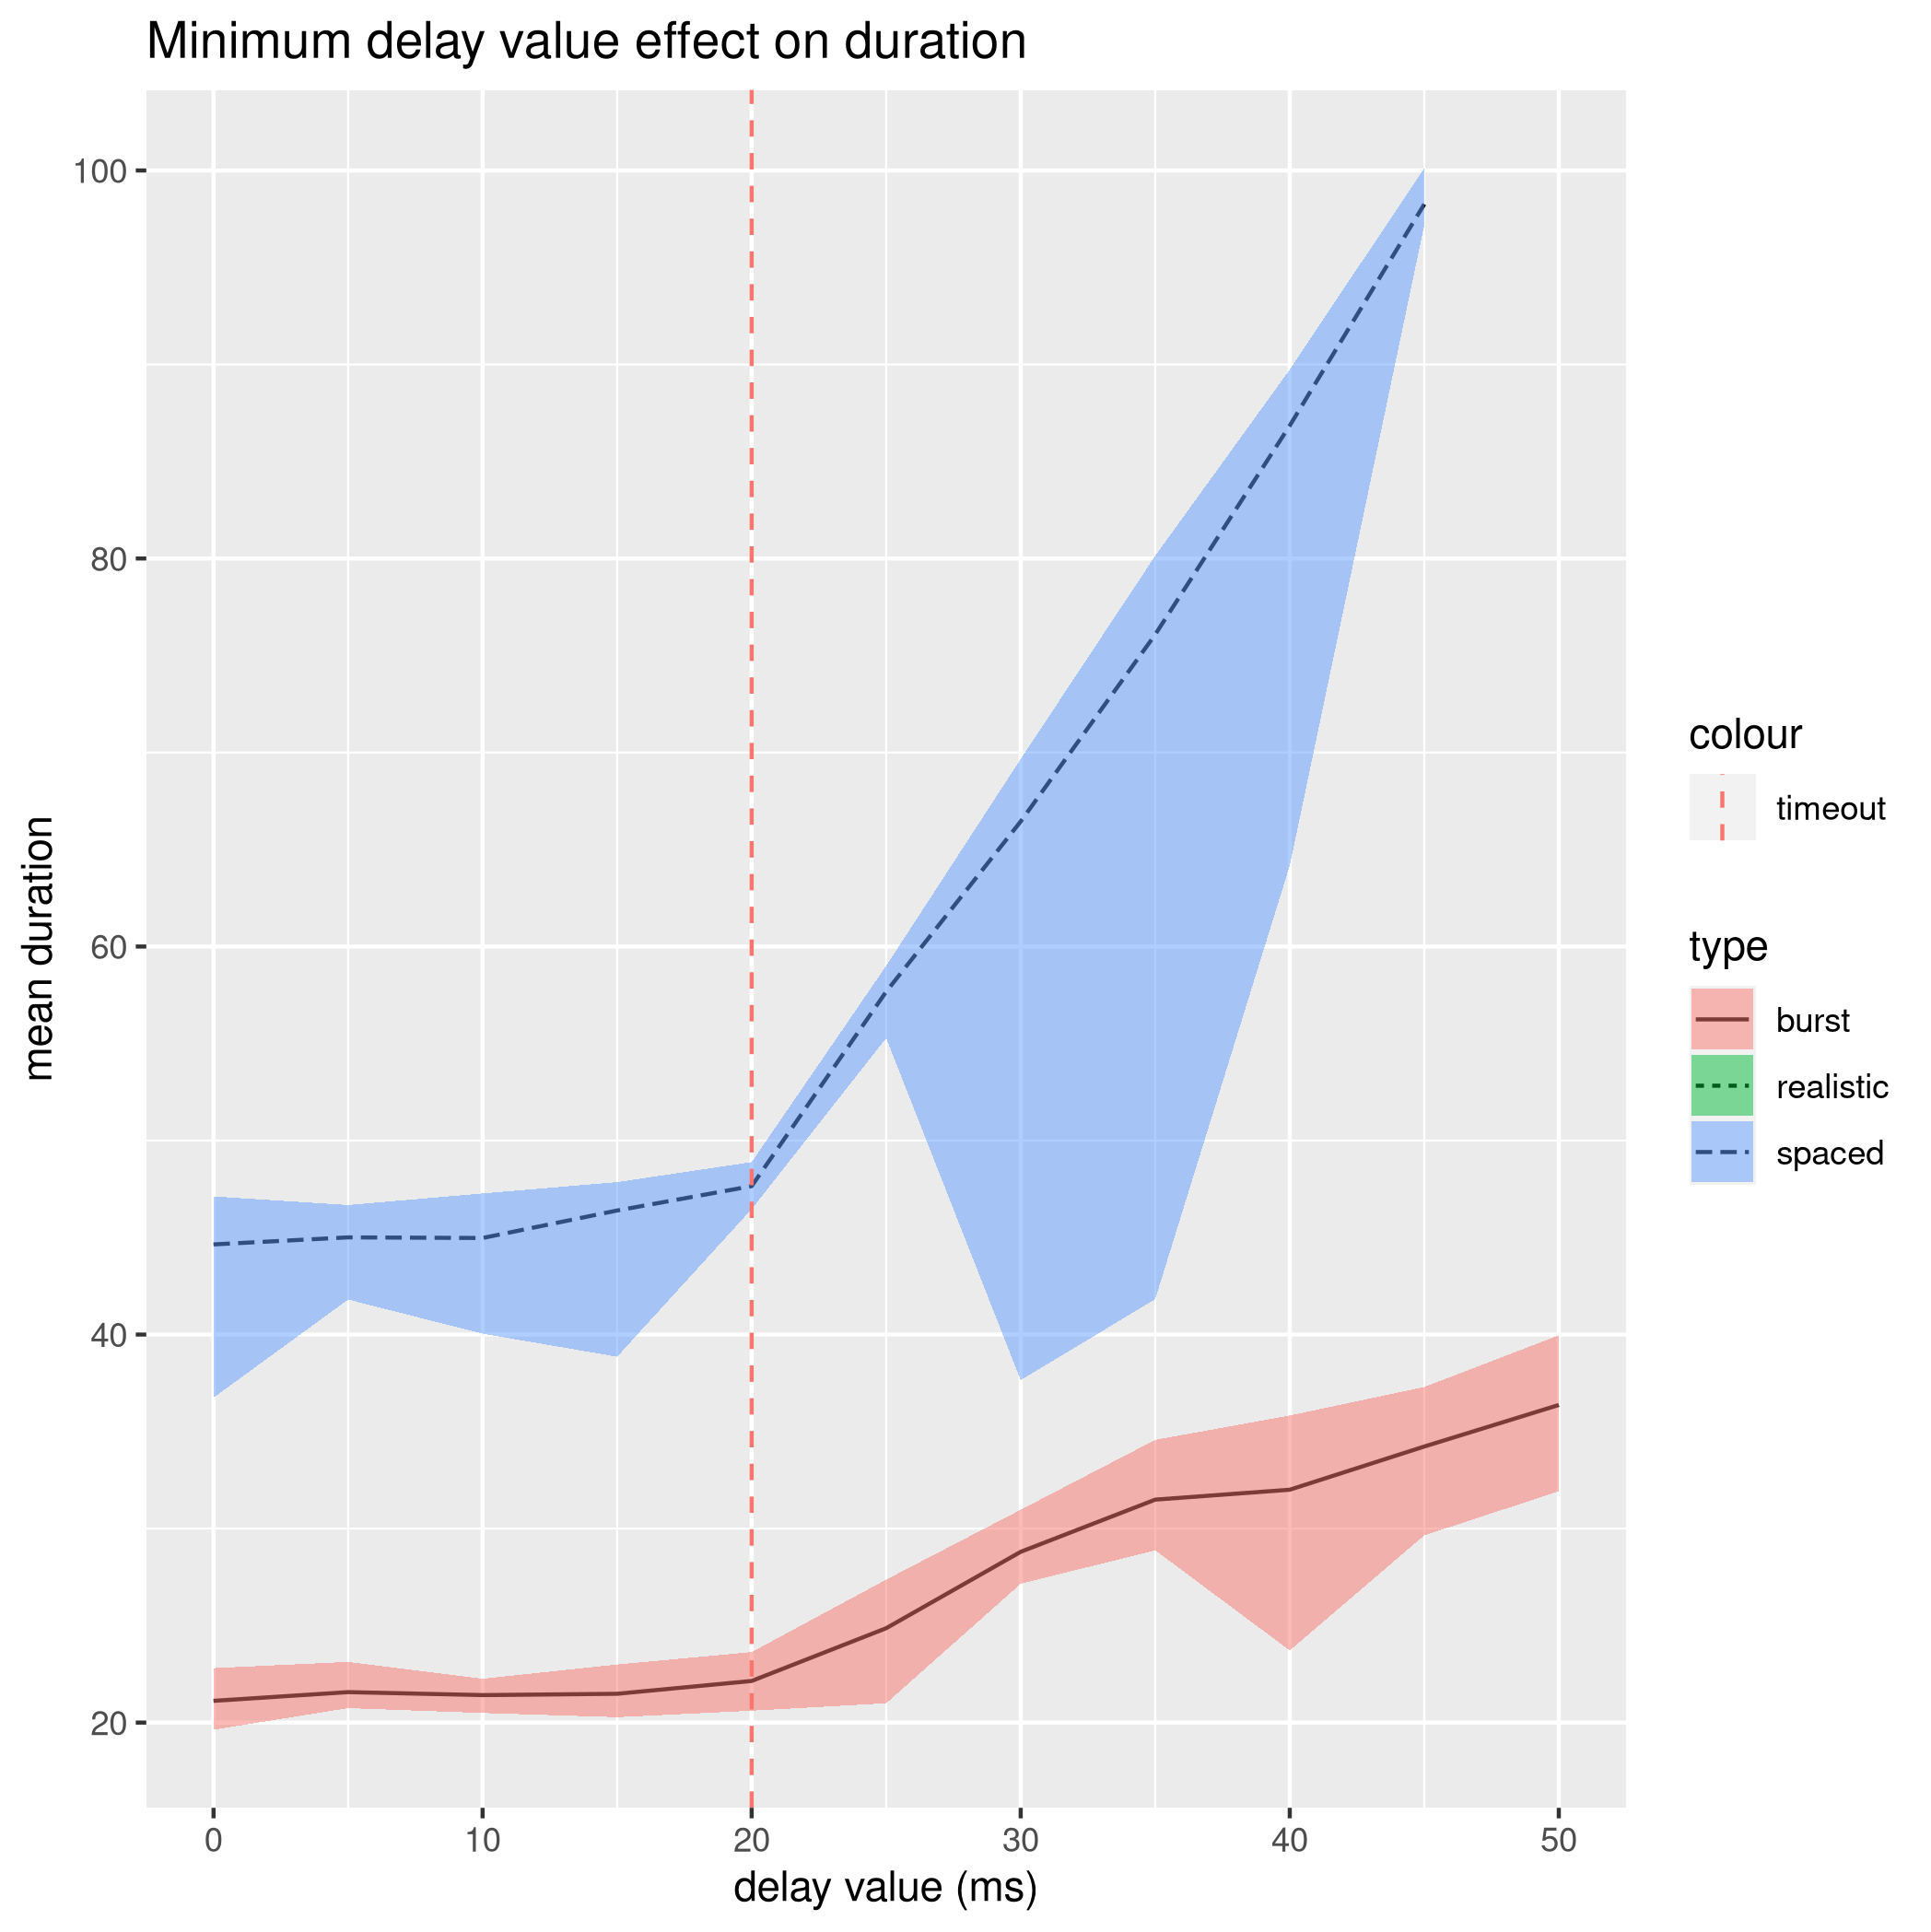
\includegraphics[width=\textwidth]{imgs/min-delay_duration.png}
	\caption{Mean duration of the simulations (in case of success) against minimum delay. Error bars show confidence intervals at 95\%.}
	\label{fig:min-delay_duration}
\end{figure}

As we can see on figure \ref{fig:min-delay_crash}, the crash rate decreases
dramatically as soon as the minimum delay reaches a certain threshold, which
here is 10ms.  This crashing issue though was resolved with an update of the
scheduler : the success rate flattens out at 100\% -- or around 100\%. Then,
with earlier versions of the scheduler, the user may have to adjust the minimum
delay in order to run simulation smoothly. 

We also observe on figure \ref{fig:min-delay_duration} -- which was made with
an updated scheduler -- a prompt increase in simulation time from delay value
20ms. This is due to the fact that the \textit{timeout} value is 20ms, which is
reached most of the time because the vast majority of the calls to the
scheduler do not result in a decision making. After this value, we notice a
direct correlation between \textit{minimum delay} increase and simulation time
increase. It follows that the best choice for the \textit{minimum delay} now is
zero, and we will use this value for the rest of the experiments.


\subsection{Timeout}

This value is the maximum amount of time we leave for the scheduler to react. A
\texttt{timeout value} not large enough may lead to inaccuracies in the
simulation: for example, if the scheduler needs 30ms to make a decision upon
reception of a message, and the value of the timeout is 20ms, Batkube will
receive the decision on the next cycle which may happen several dozens of
seconds later (depending on the \textit{maximum simulation time step} value).
On the other hand, a \textit{timeout value} too large will induce longer
simulation times. Indeed, once the simulator was given enough
time to process a message, any time following is spent idling. We want to
measure which \texttt{timeout value} is just enough for the scheduler to be
able to make a response without spending any time idling.

We run each workload with a \texttt{timeout value} ranging from 0ms to 100ms,
with a step of 1ms. Each time we measure the duration of the simulation as well
as the makespan and the mean waiting time. The latter two will enable us to
compare the results against the emulated results in order to estimate the
accuracy of the simulation. The other parameters are set to:
\texttt{min-delay=0ms}, \texttt{max-simulation-timestep=20s}

\begin{figure}
	\begin{subfigure}{.5\textwidth}
		\centering
		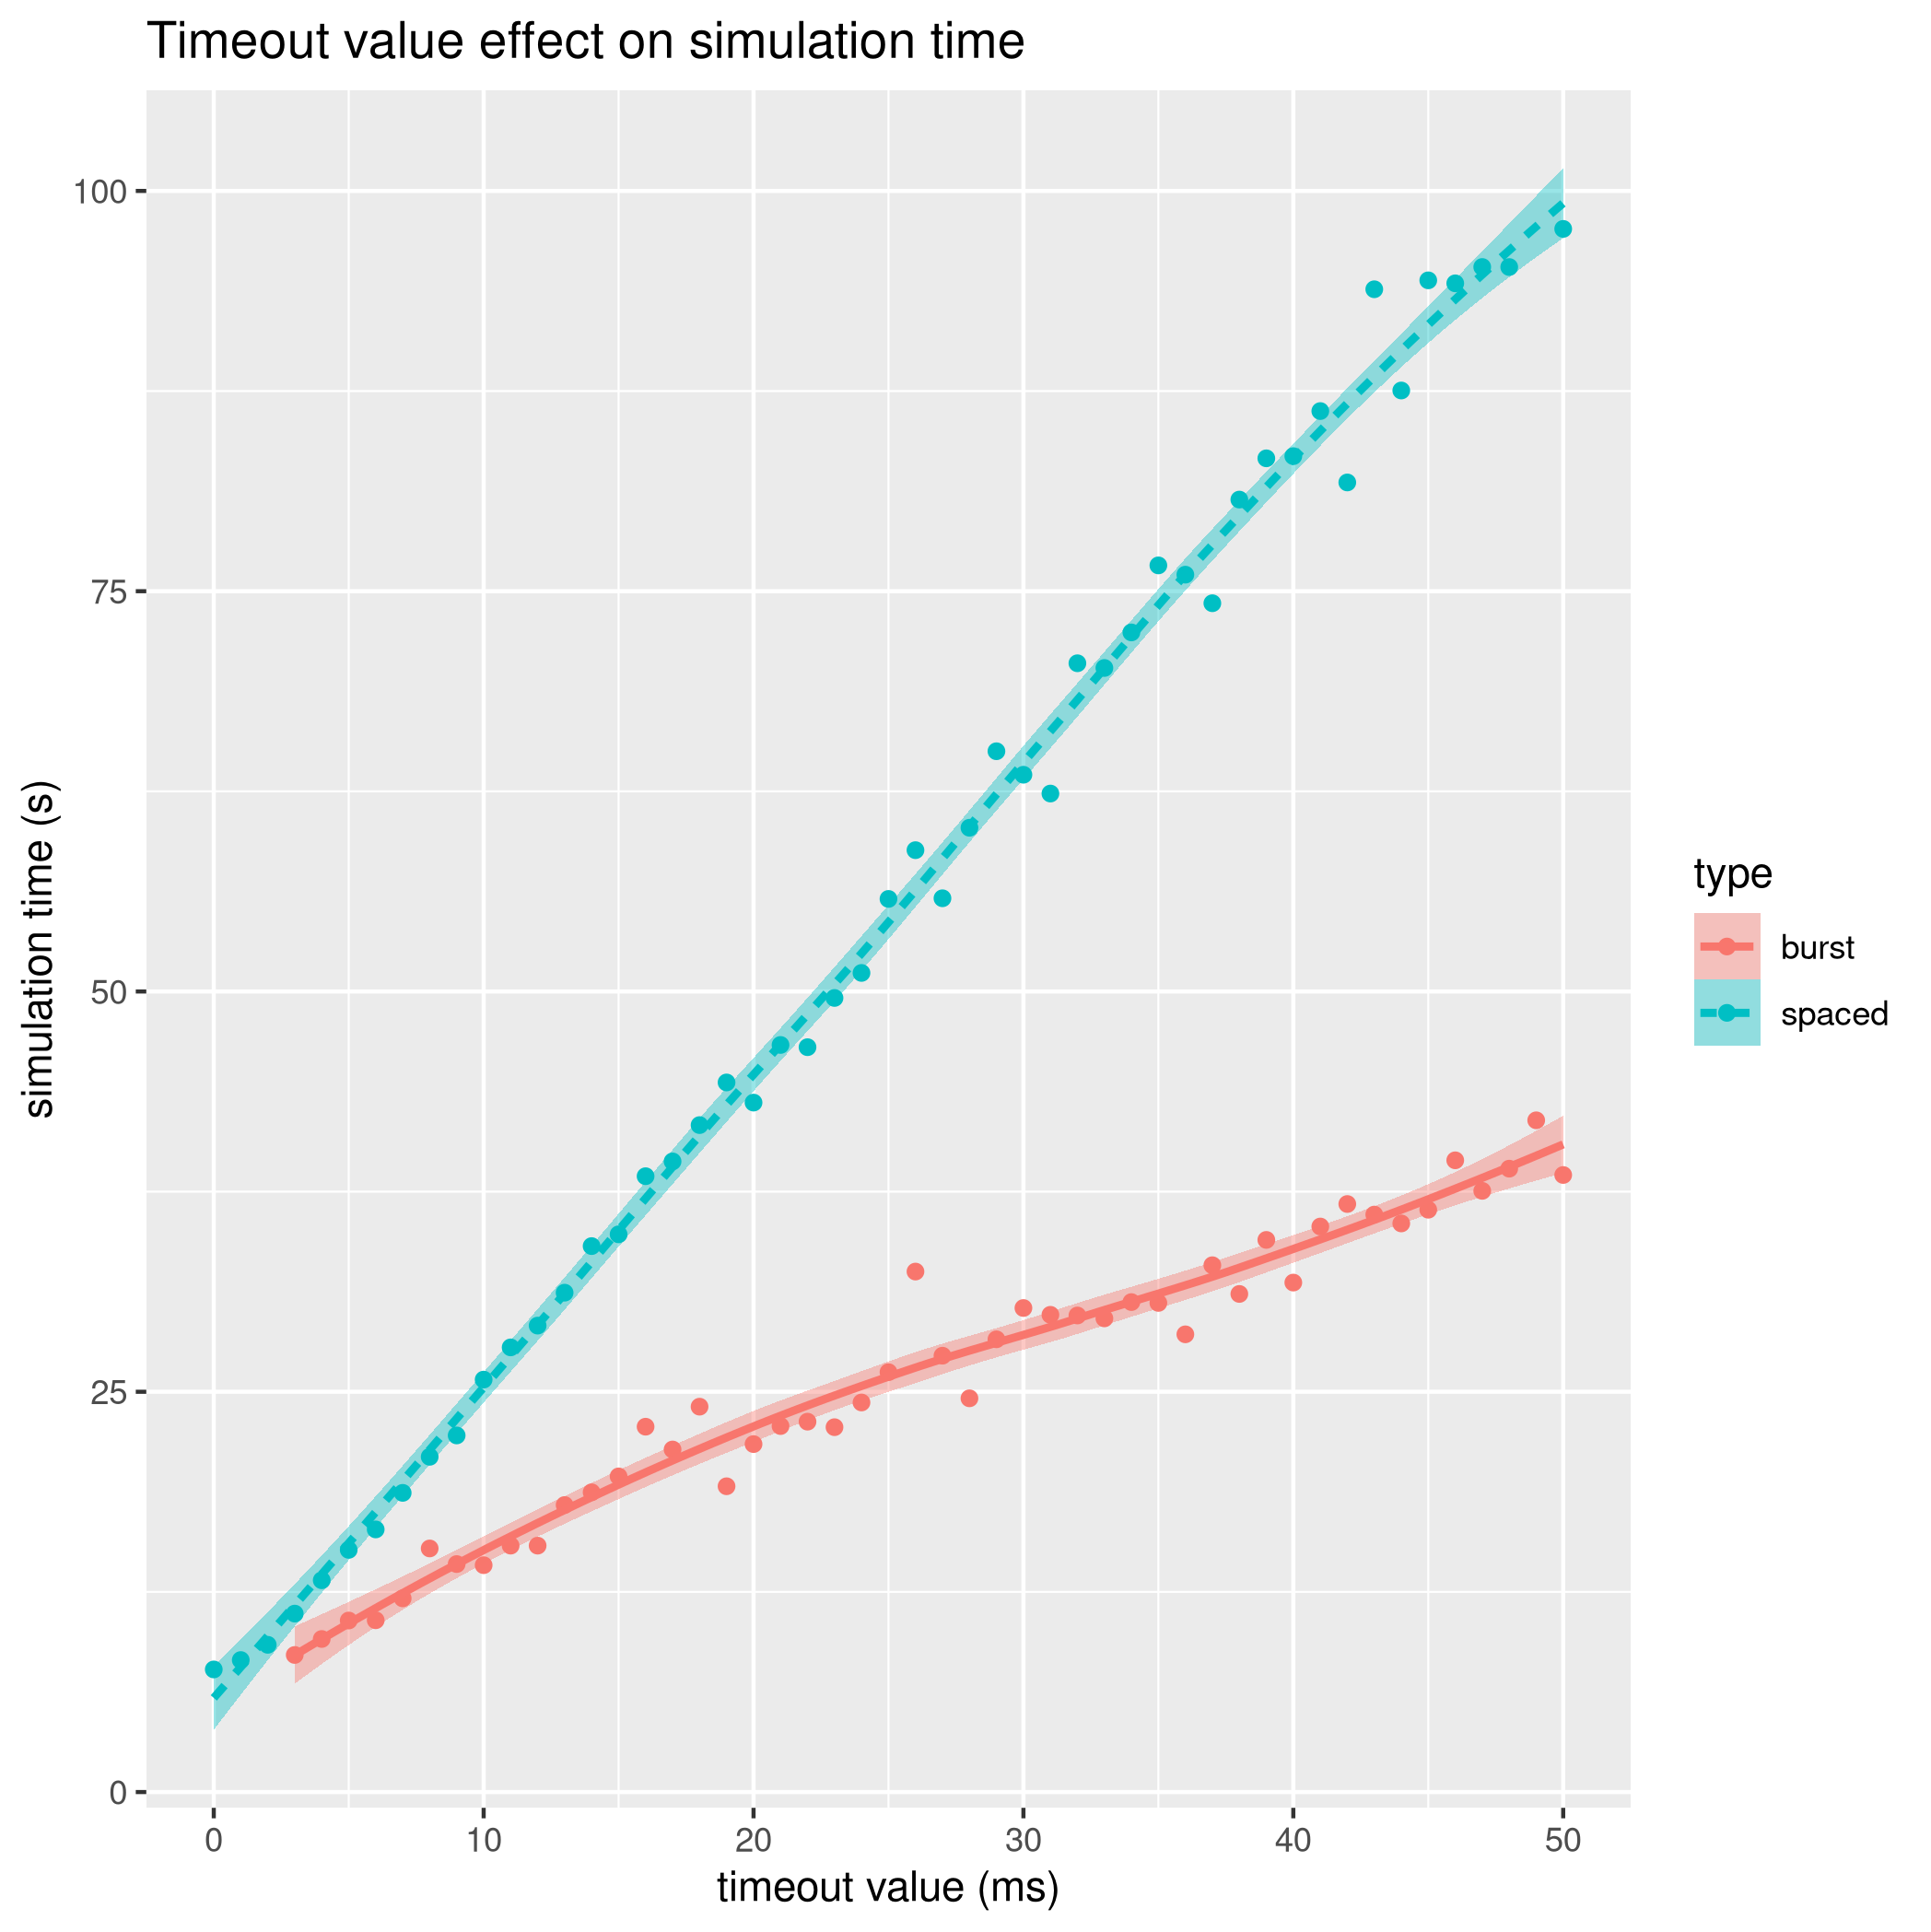
\includegraphics[width=\linewidth]{imgs/timeout_duration.png}
		\caption{}
		\label{fig:timeout_duration}
	\end{subfigure}
	\begin{subfigure}{.5\textwidth}
		\centering
		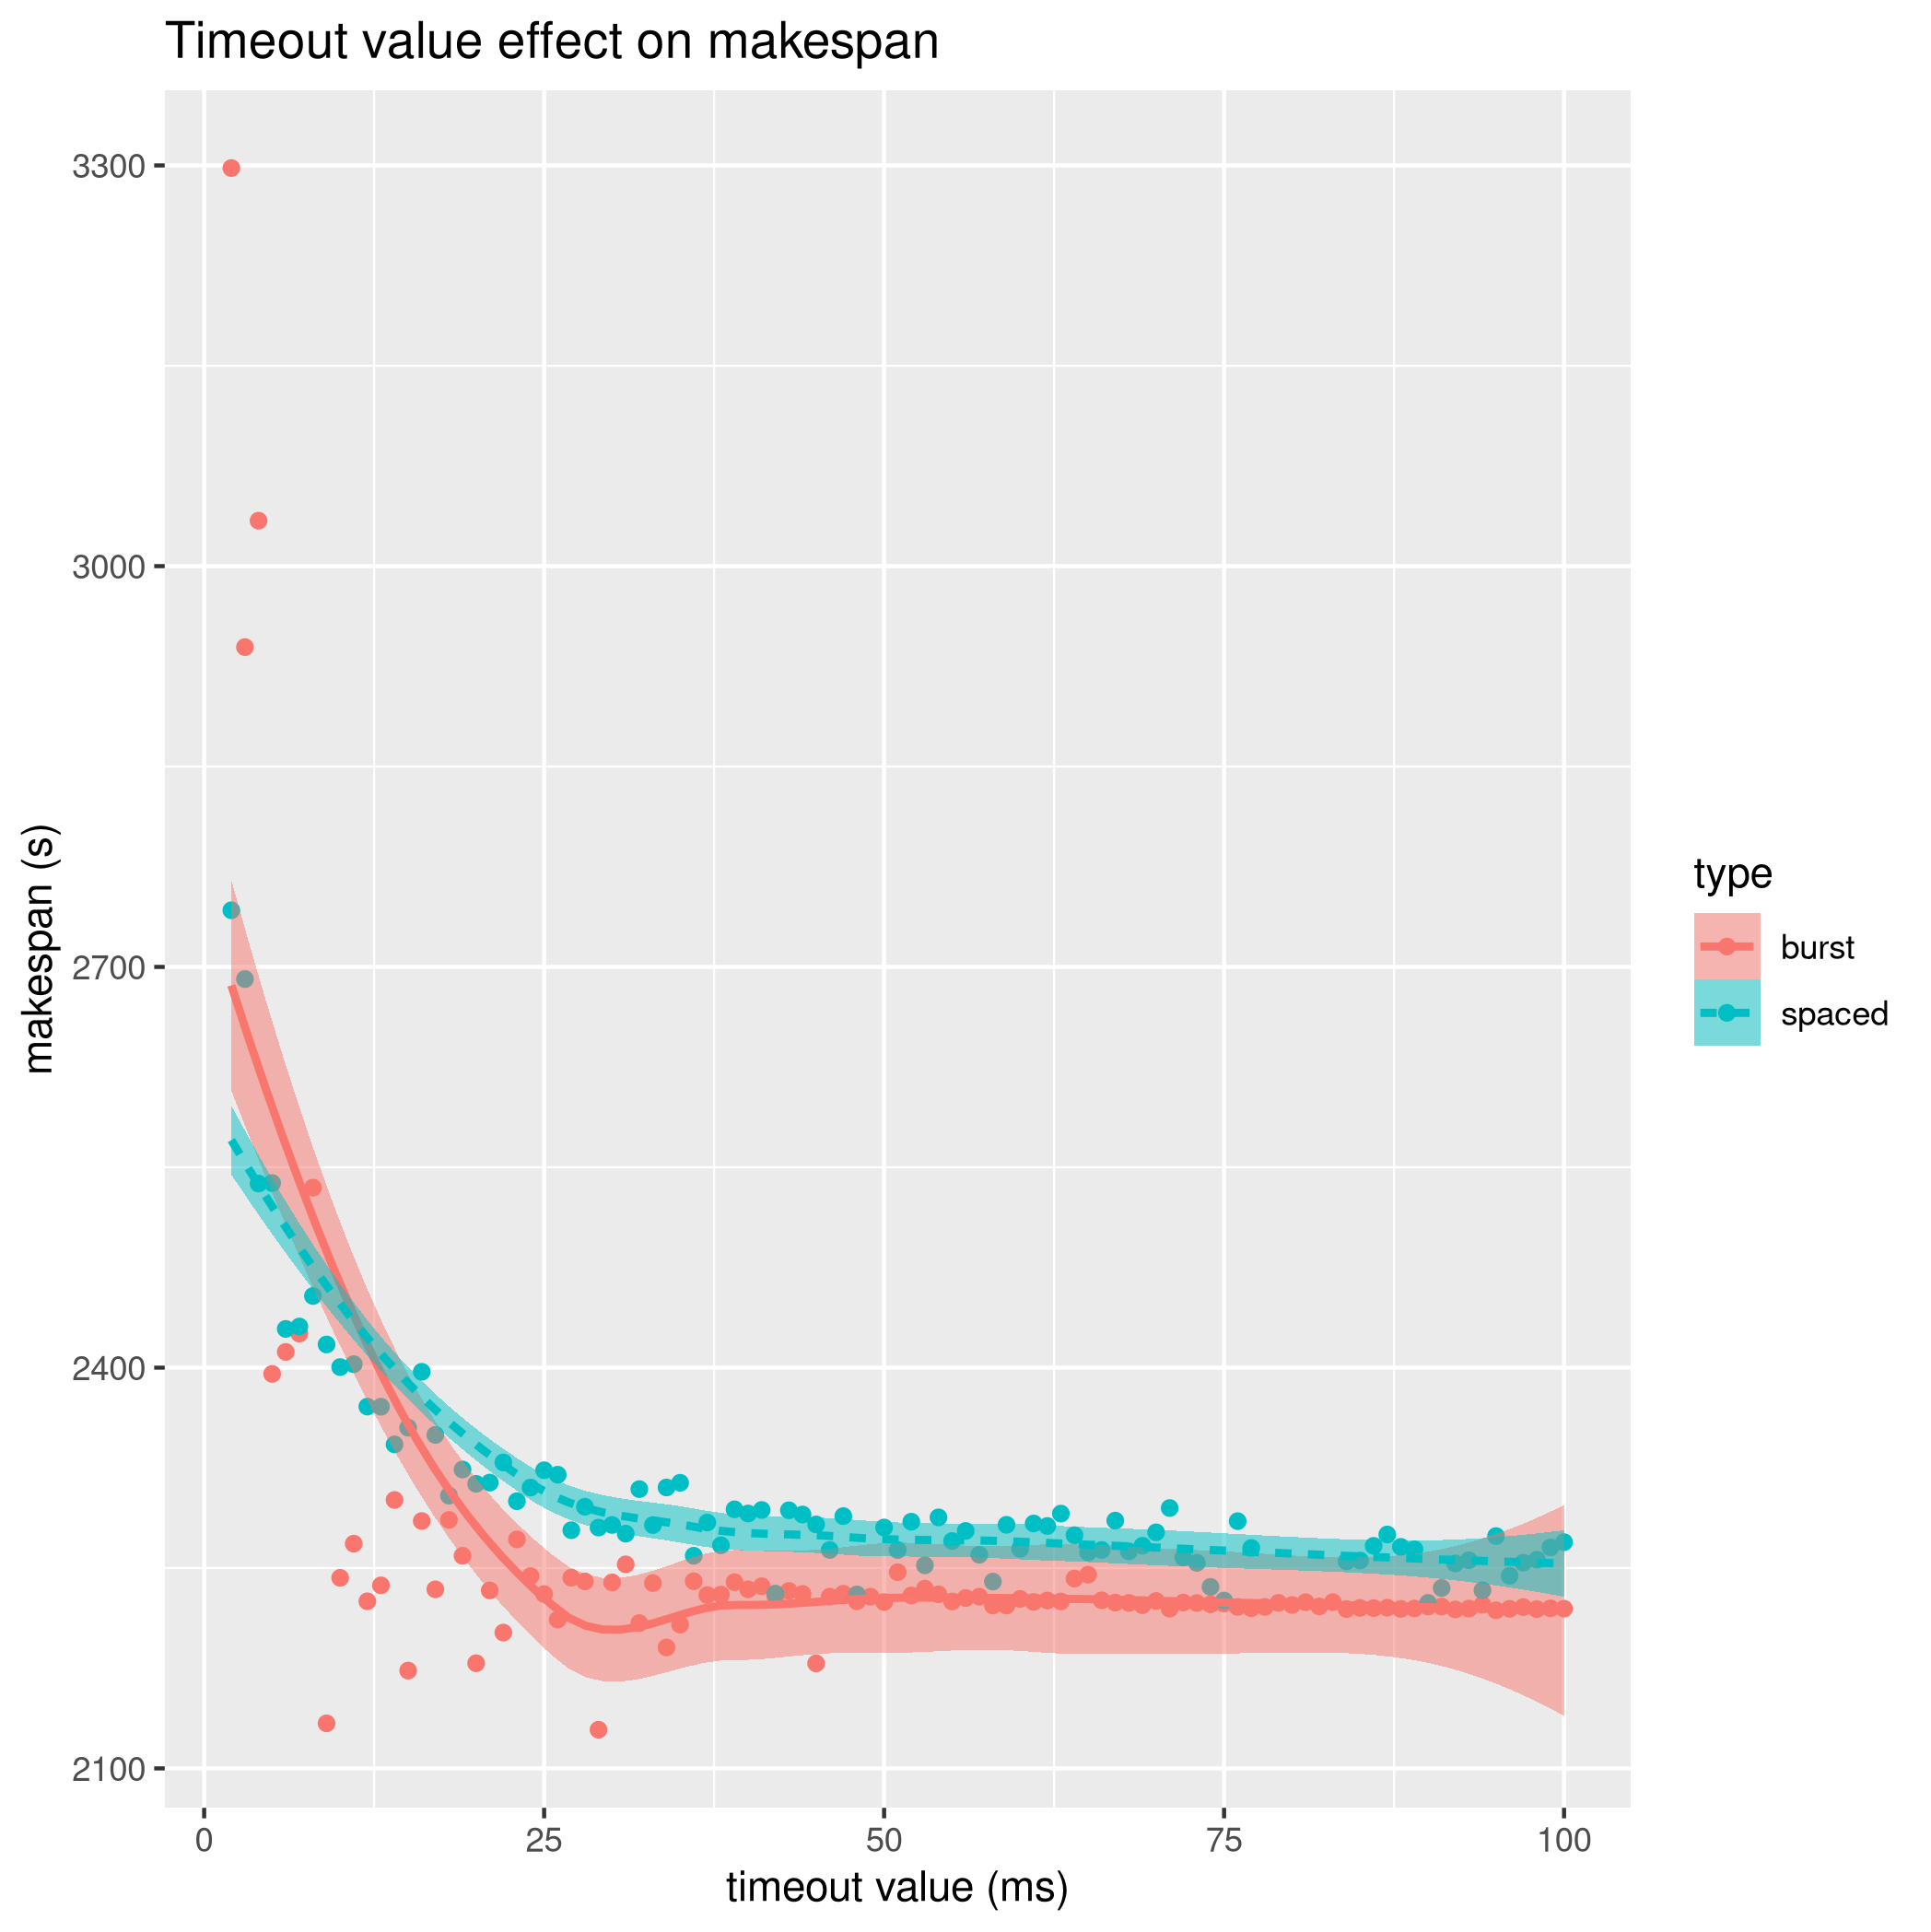
\includegraphics[width=\linewidth]{imgs/timeout_makespan.png}
		\caption{}
		\label{fig:timeout_makespan}
	\end{subfigure}

	\centering
	\begin{subfigure}{.5\textwidth}
		\centering
		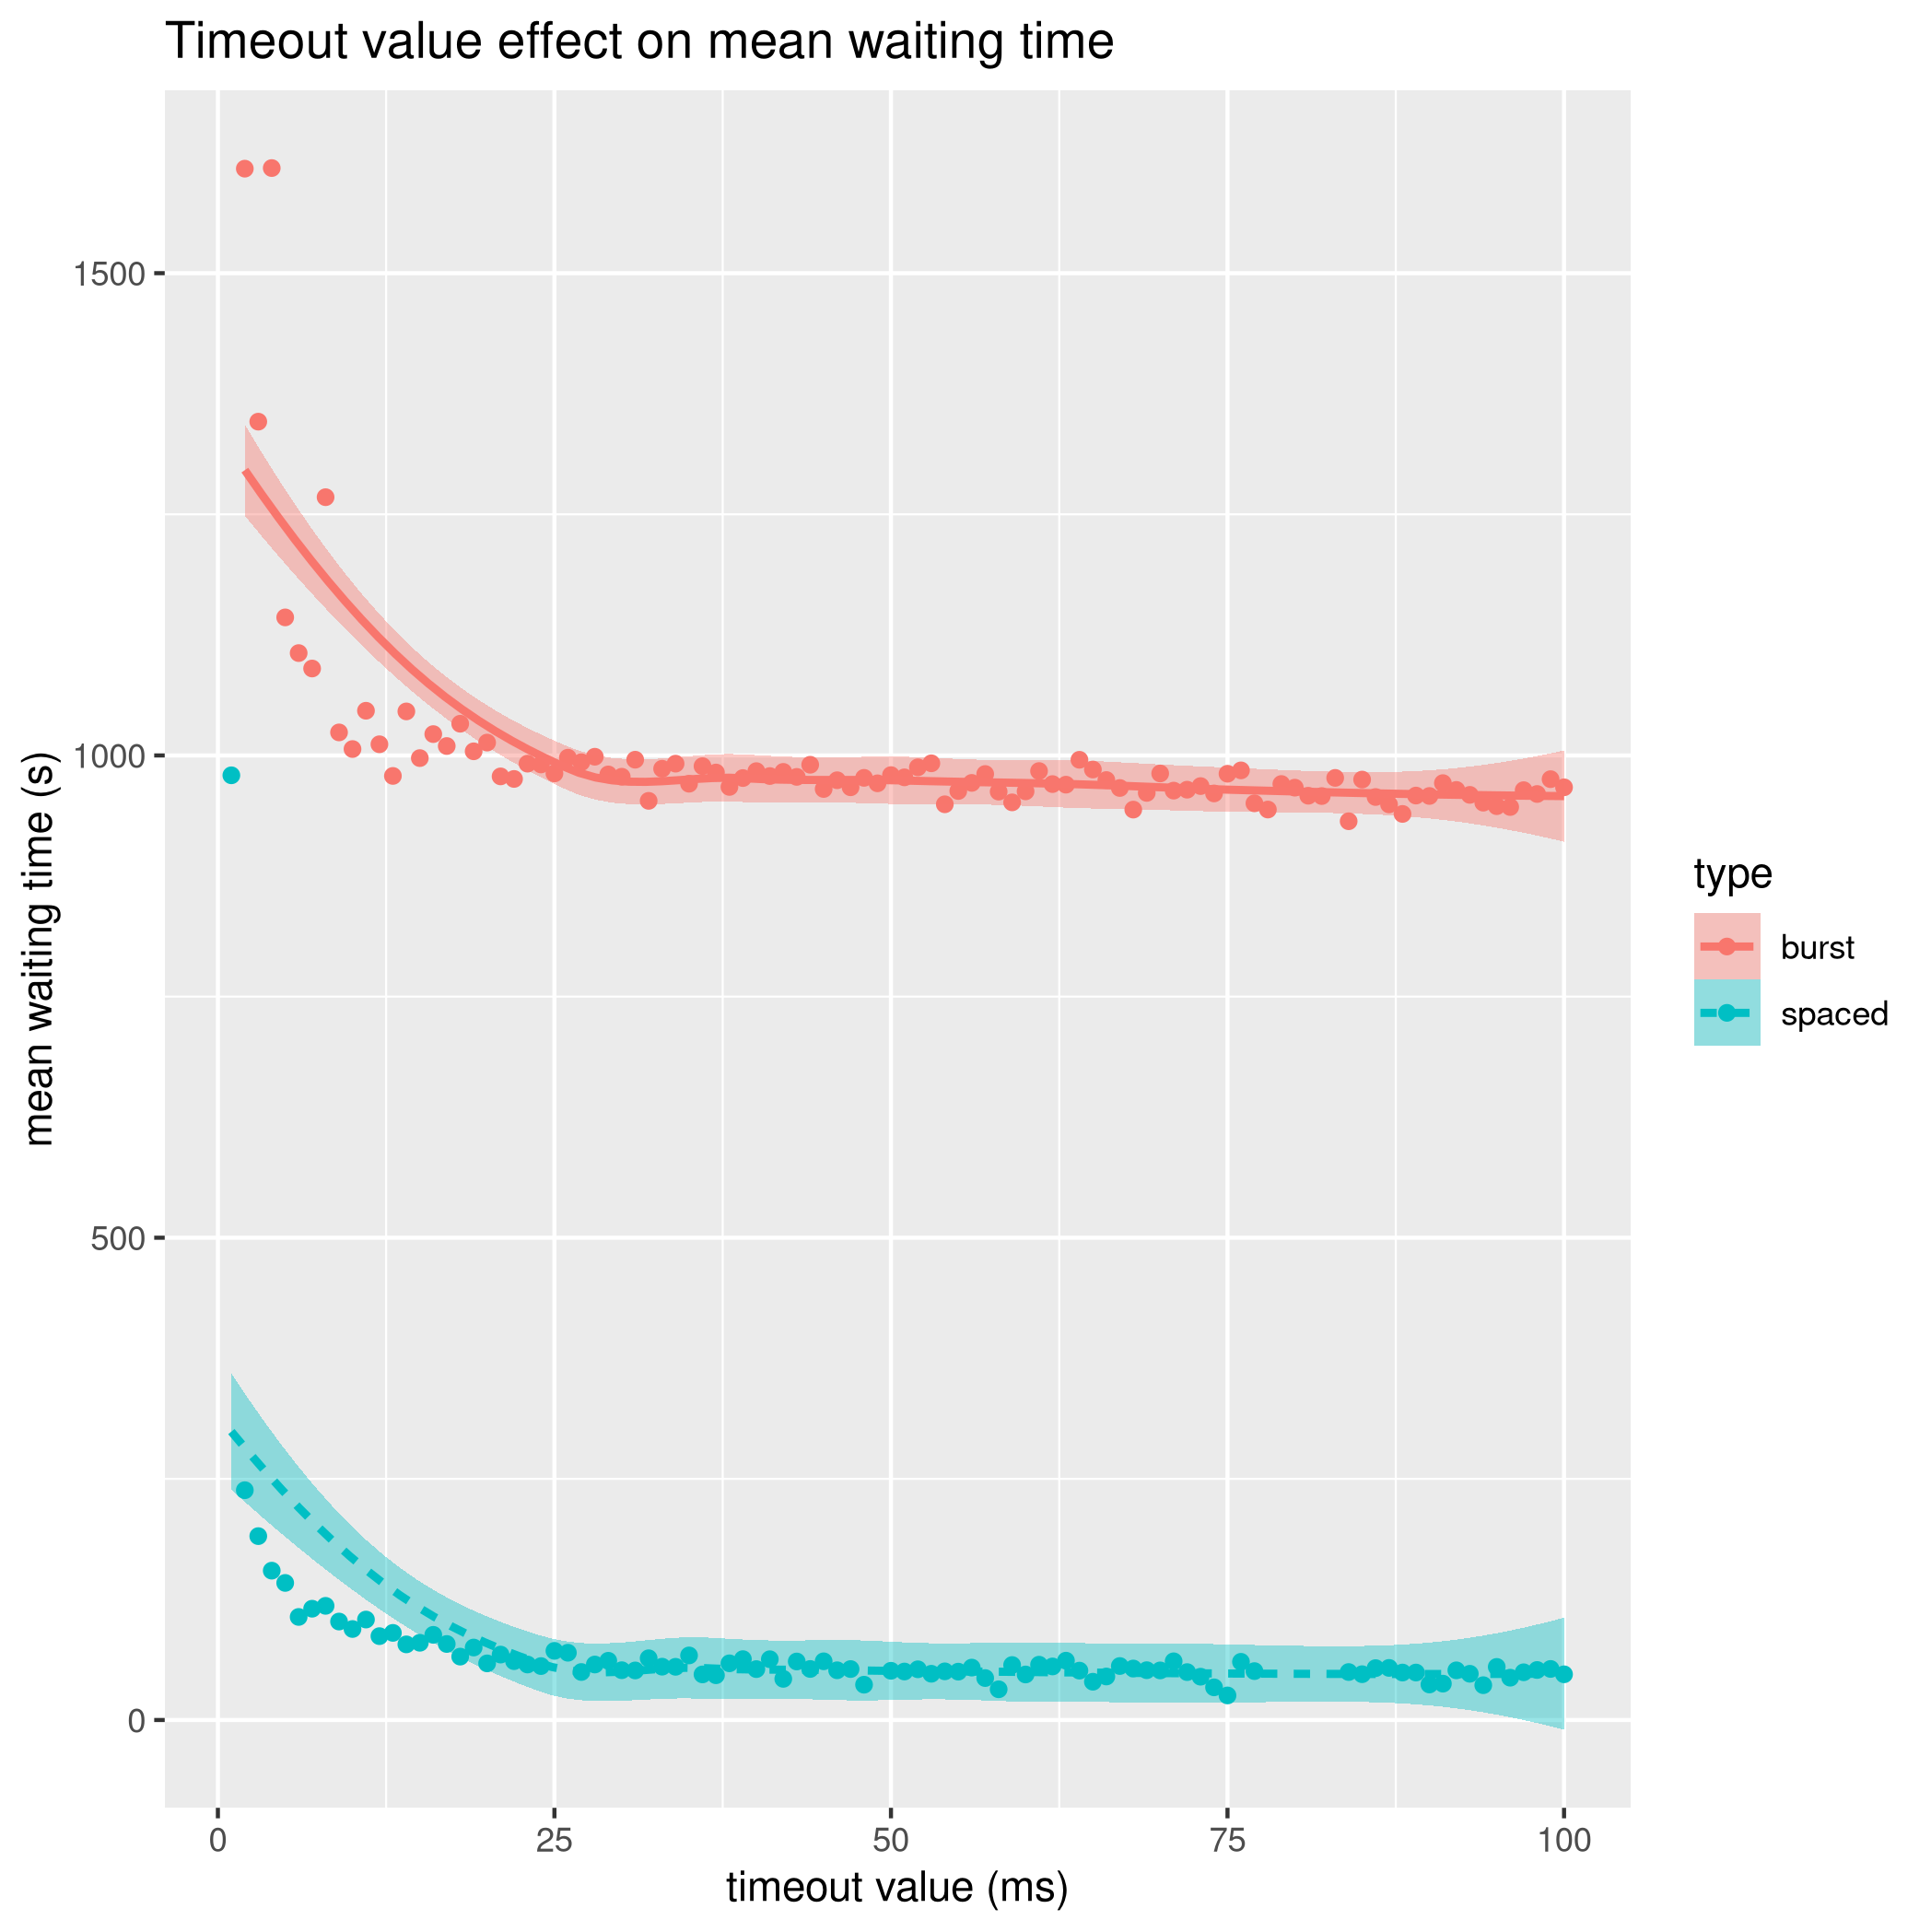
\includegraphics[width=\linewidth]{imgs/timeout_mwt.png}
		\caption{}
		\label{fig:timeout_mwt}
	\end{subfigure}
	\caption{Effect of the timeout value on the simulation}
	\label{fig:timeout}
\end{figure}

TODO: redo the simulations for the realistic wl, removing some values of
timeout and adding repetition to show aggregated metrics. (non aggregated ones
are too dispersed)

TODO: \ref{fig:timeout_duration} does not have the same scale on the x axis as the others.

TODO: Gantt charts to show the gaps.

As we expected, a \textit{timeout value} too low results in the scheduler
missing a few cycles each time it wants to communicate a decision making, thus
increasing the makespan and mean waiting time.  As the \textit{timeout}
increases, it reaches a point where the scheduler consistently sends decisions
in the same cycle as the one where it has received the message that triggered
the decision making. After this point though the curves keep decreasing,
showing that the gaps keep receding afterwards. However, the gain in accuracy
is shallow and considering that there is, again, a direct correlation between
the \textit{timeout value} and the simulation time, it is desirable to keep
this value at the limit where the results start to stabilize.  In this case,
according to figure \ref{fig:timeout_makespan}, \texttt{timeout-value=50ms}
seems like a decent compromise between accuracy and scalability.

With such simple workloads and platforms, the decision making time is very low
(it is but a matter of milliseconds), but we can imagine it may reach much
higher values given a bigger platform and more complicated workload.

\subsection{Maximum simulation time step}

Having a high maximum time step value will allow Batsim to jump forward further
in time. This may result in skipping scheduler decisions that could have been
made in the mean time, delaying them to when Batsim decides to wake up. We
expect increasing this value to have an analogous effect to the timeout value:
higher simulation speed, but also decreased accuracy due to gaps (delays) in
the decision process.

To experiment with the maximum time step effect on the results we obtain, we
run each workload with different values of \texttt{max-simulation-timestep}
following a logarithmic scale. The other parameters are fixed to
\texttt{min-delay=0s}, \texttt{timeout=50ms}. Also, the
\texttt{base-simulation-timestep} was lowered to 10ms in order to test lower
values of the maximum timestep (compared to the previous 100ms).

\begin{figure}[]
	\centering
	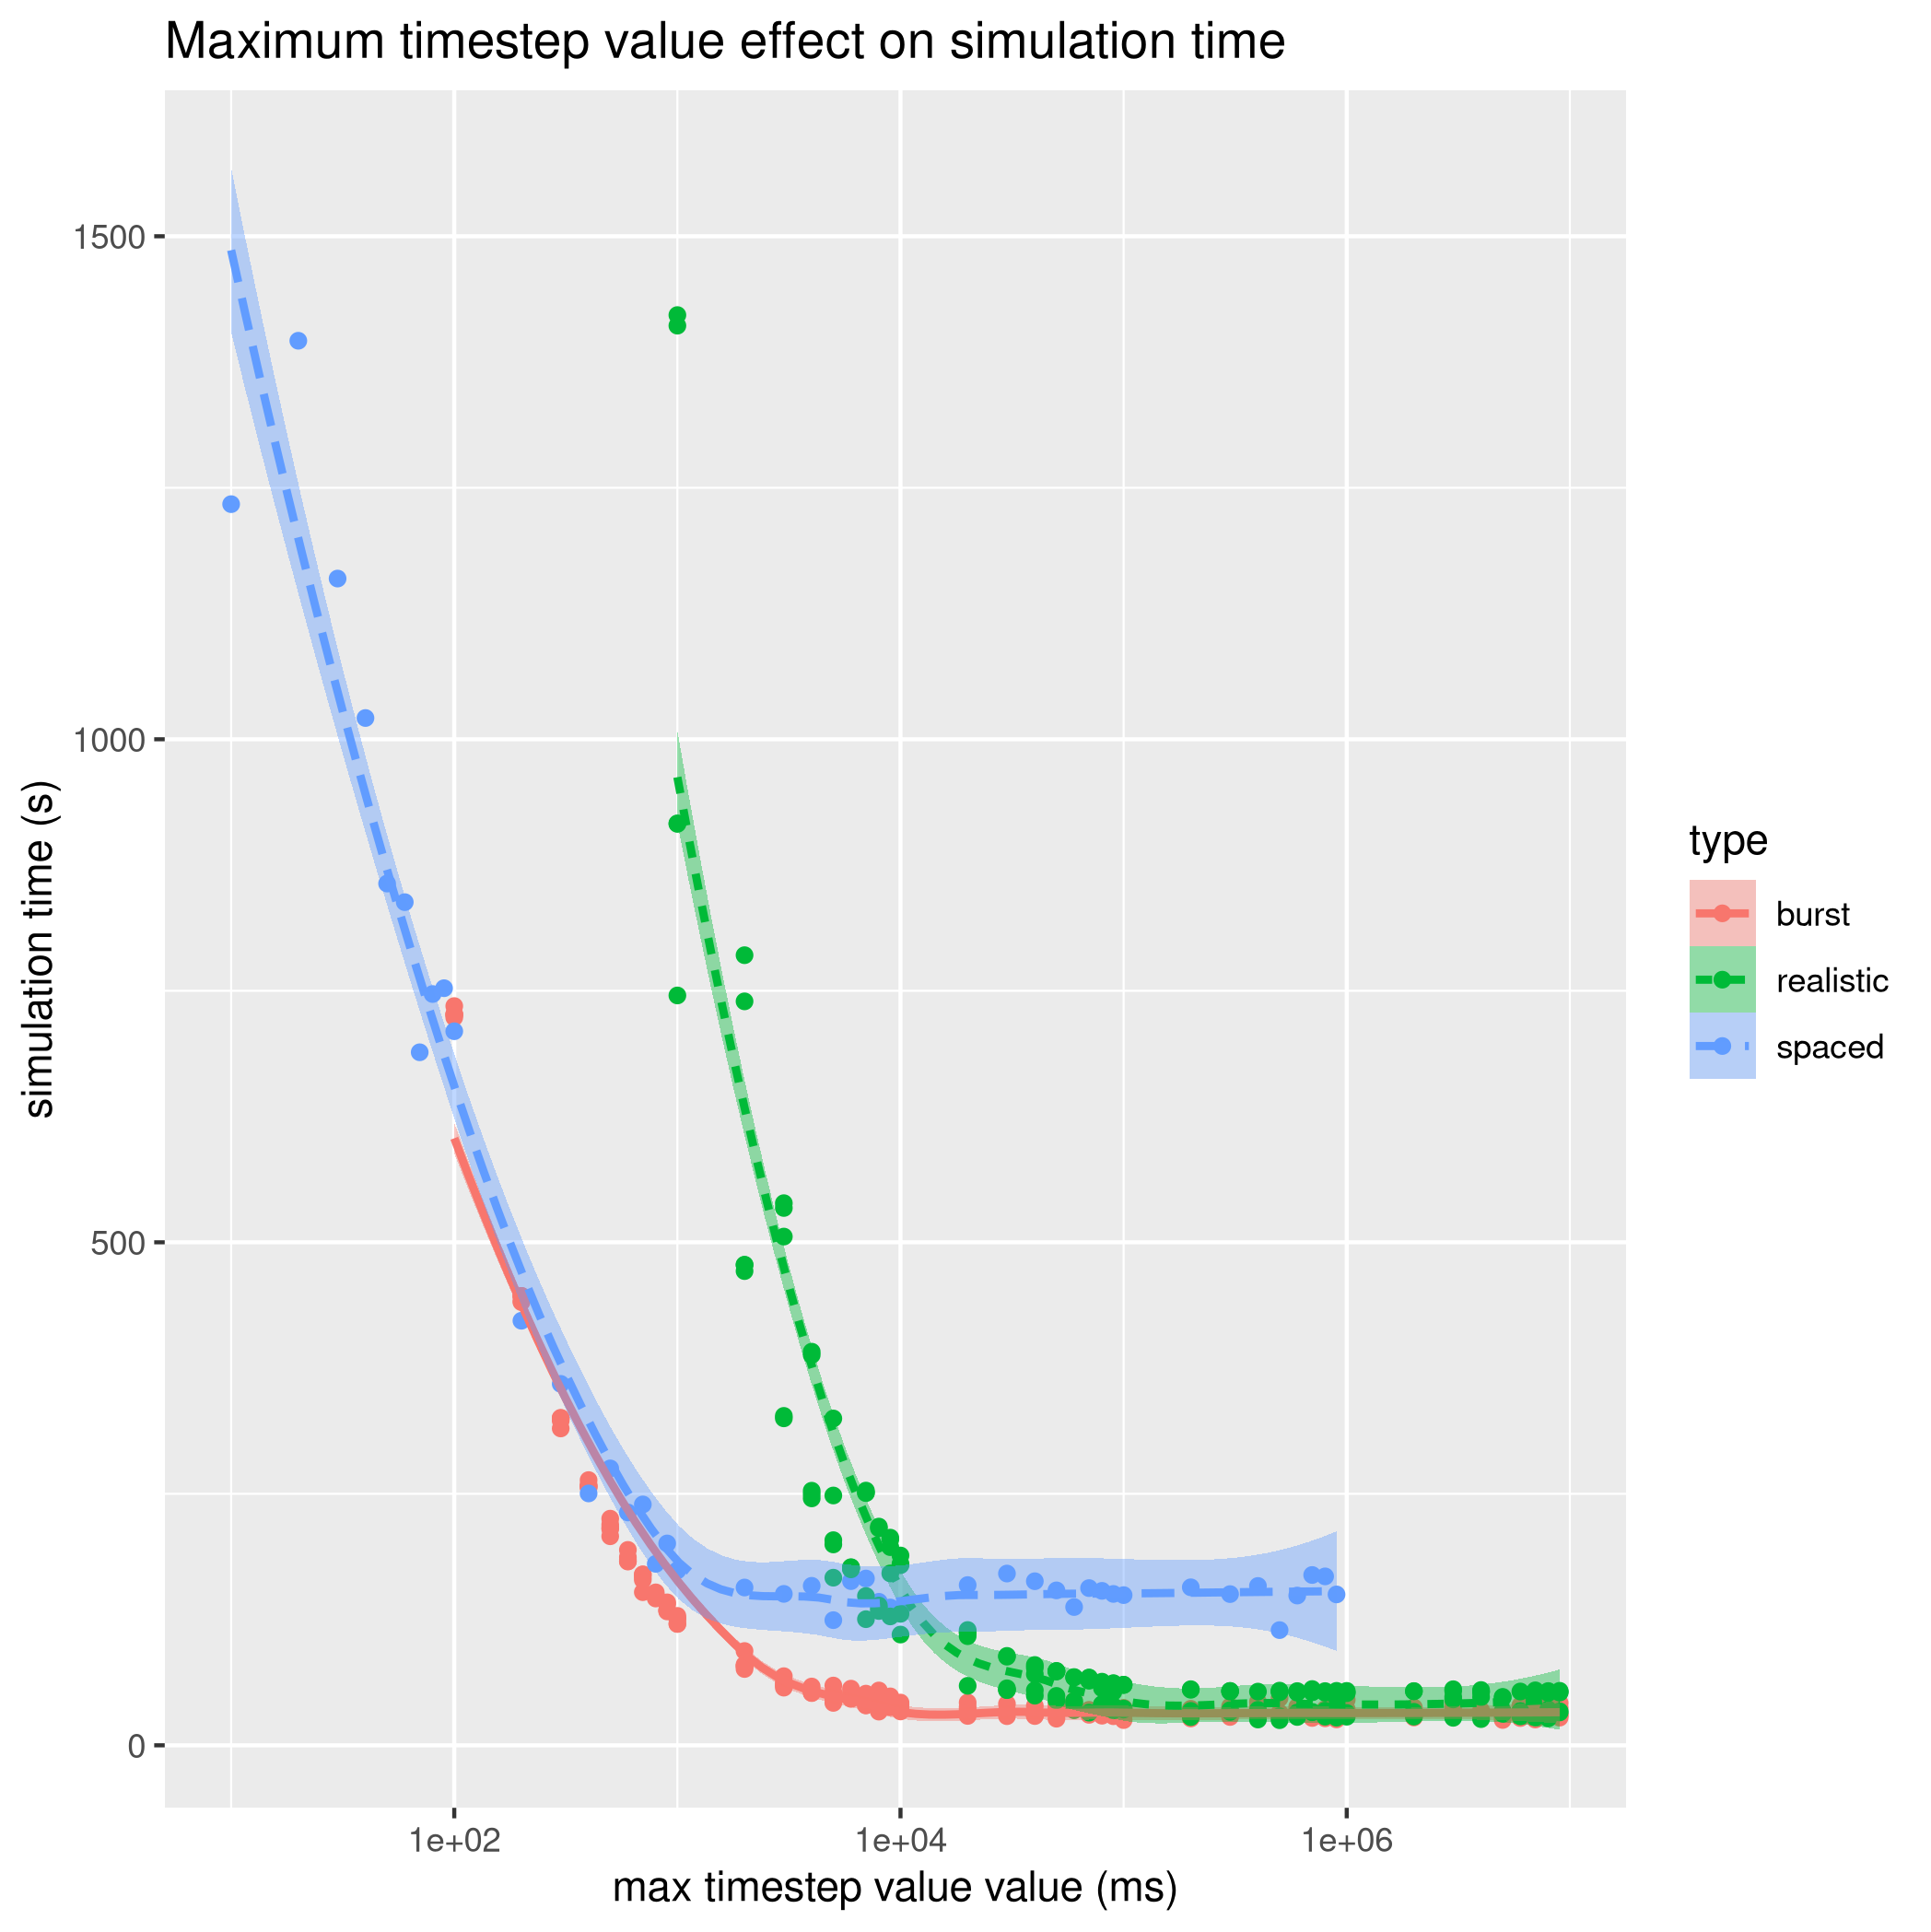
\includegraphics[scale=0.5]{imgs/max-timestep_duration.png}
	\caption{Effect of maximum timestep on simulation time}
	\label{fig:max_timestep_duration}
\end{figure}

\begin{figure}[]
	\centering
	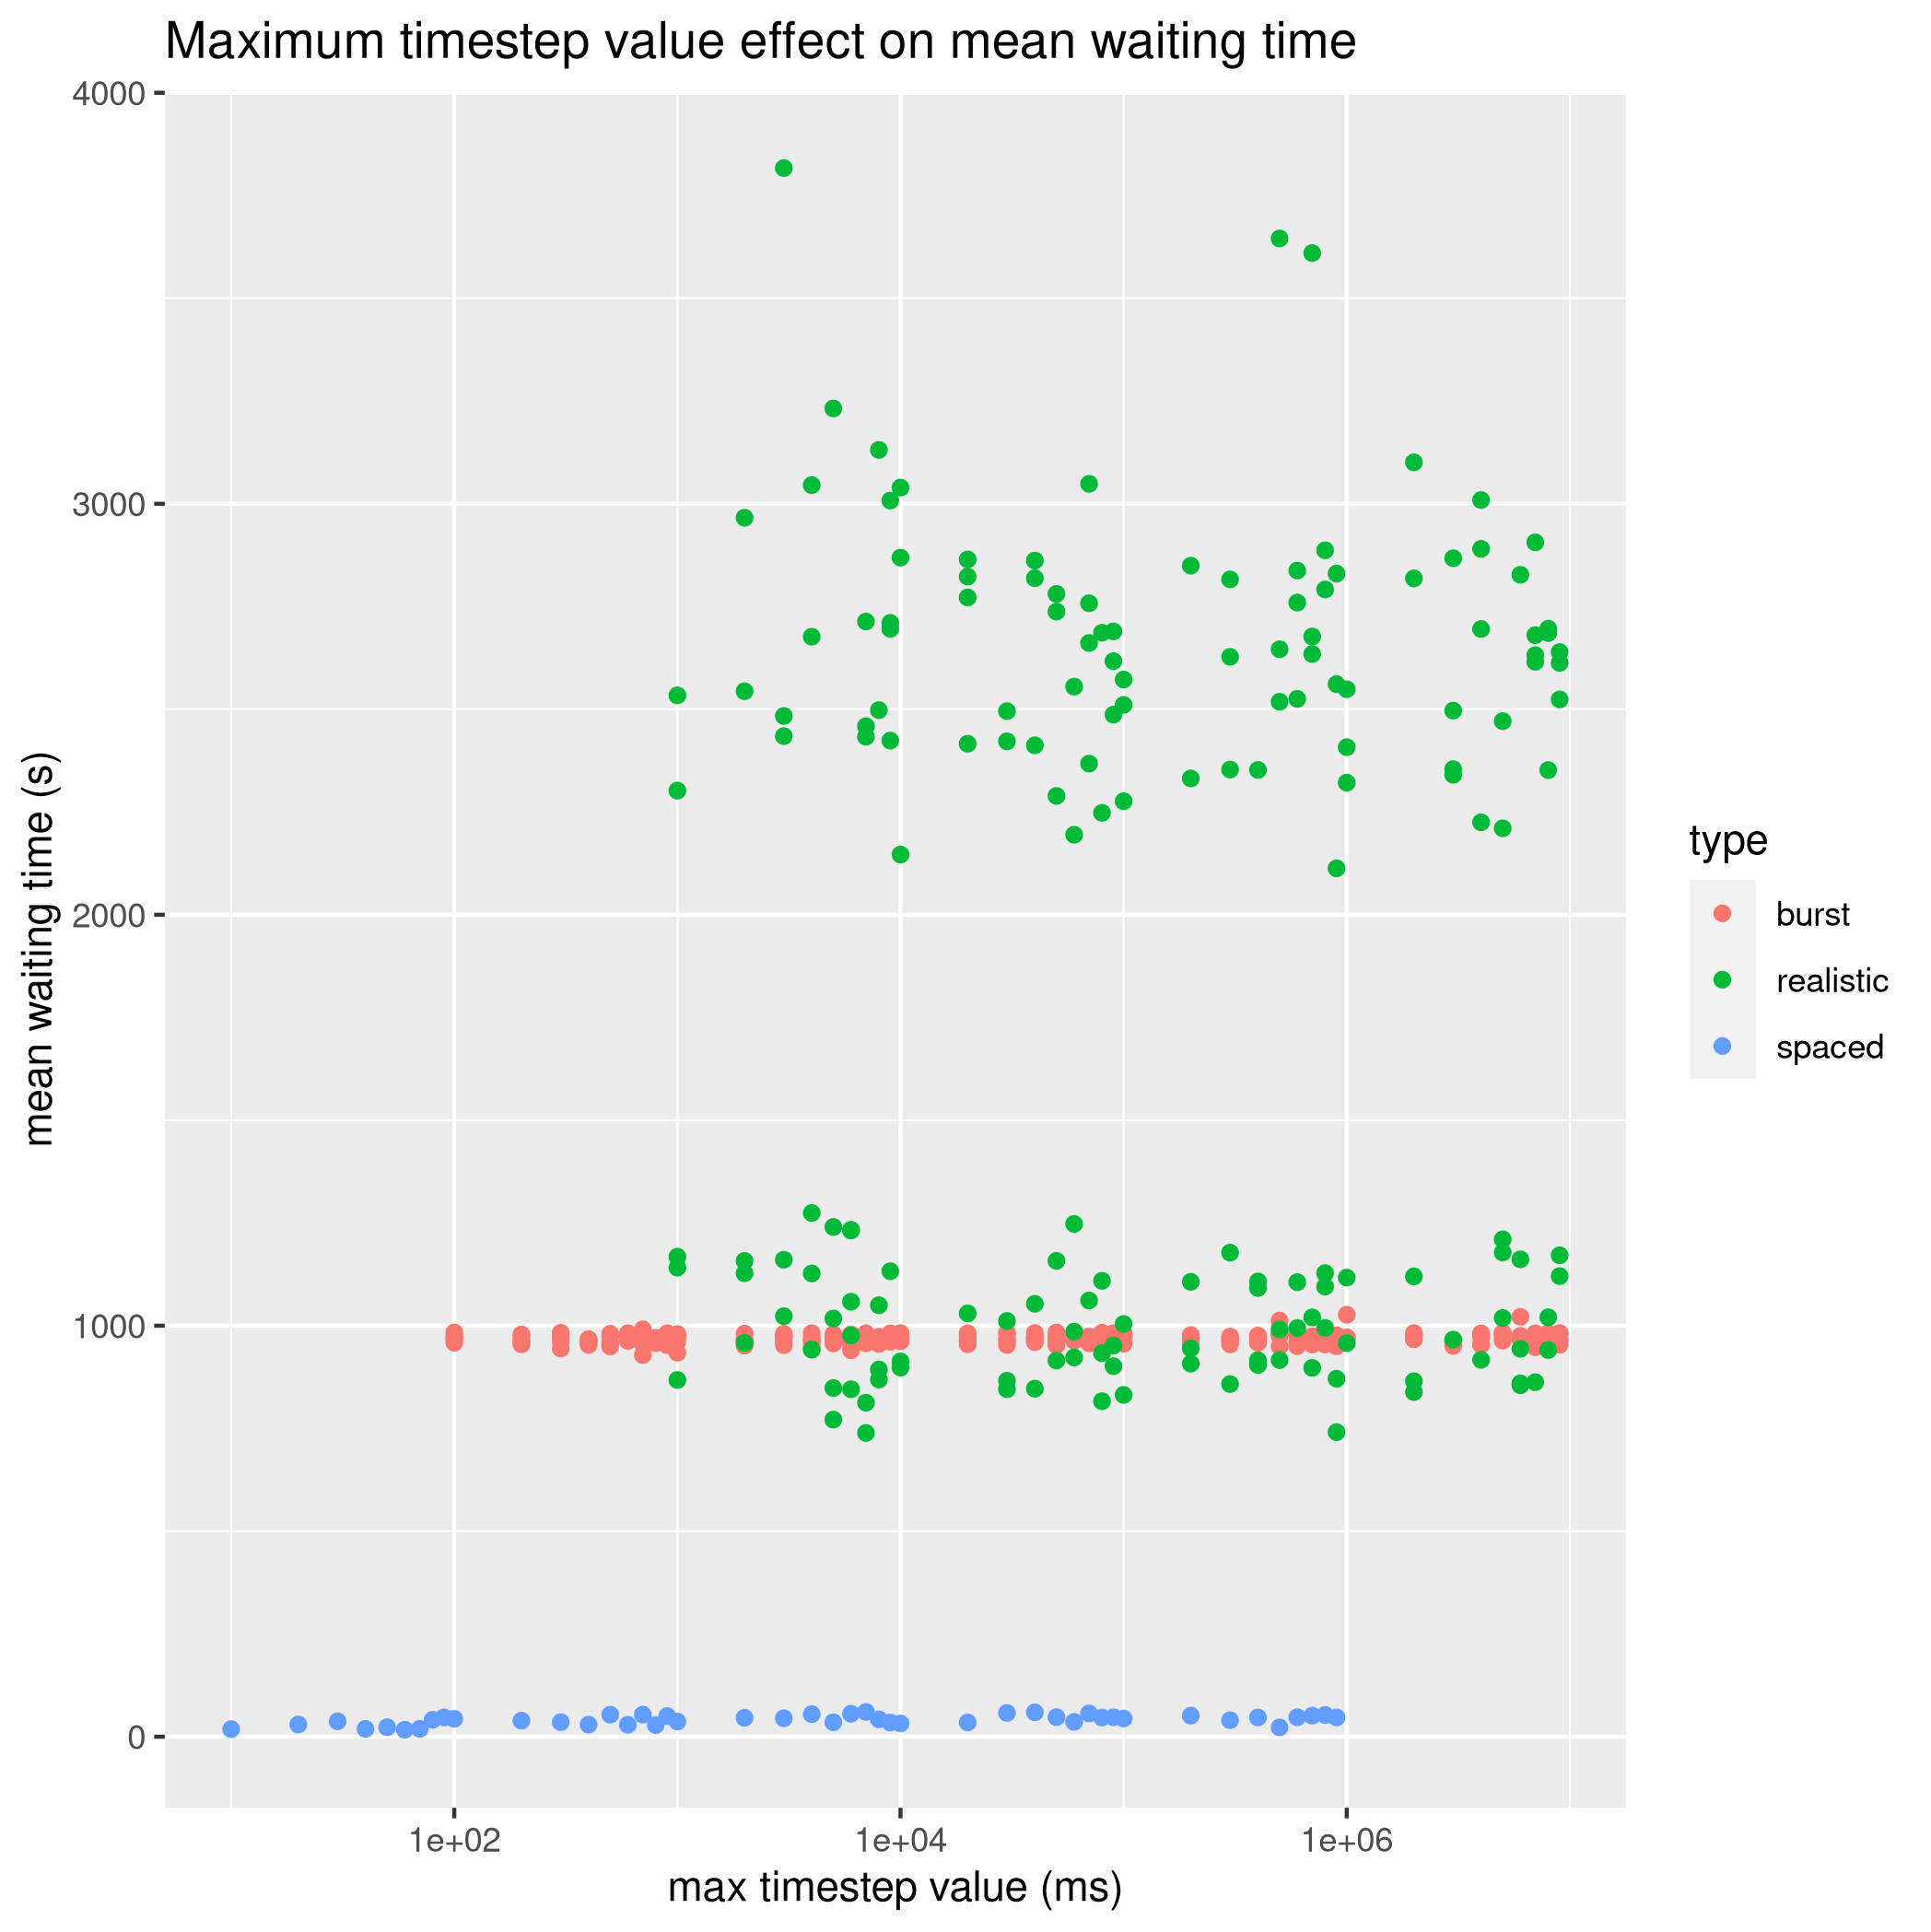
\includegraphics[scale=0.5]{imgs/max-timestep_mwt.png}
	\caption{Effect of maximum timestep on mean waiting time}
	\label{fig:max_timestep_mwt}
\end{figure}

As expected, the simulation time decreases drastically when the maximum
timestep increases. Still, this value reaches a minimum eventhough the maximum
timestep keeps increasing. This happens because Batsim events are only so far
appart in the simulation, and Batsim will always wake up before the maximum
timestep is reached.

TODO: redo the experiment for the spaced wl and redo the graph for makespan (do
not put all three wl on the same graph because the scale is so different).

\subsection{Parameters inter dependency}

Studying the parameters independently is not enough, we need to study their
impact relatively to each others.

For instance, the \textit{maximum simulation time step} and the
\textit{timeout} value are tightly linked together regarding their effect on
accuracy. Both decreasing \textit{timeout} and increasing \textit{maximum
simulation time step} will increase the amount of delays in the decision making
of the scheduler, but also their length, multiplying the impact on accuracy.

On the other hand, we do not except the \textit{minimum wait delay} to have any
impact other than increasing the simulation stability.

PROTOCOL: We know the simulations are statistically the same by now, and we're
confident enough to run only one simulation per point. Timeout value ranges
from 5ms to 50ms, max timestep ranges from 1s to 100s (logarithmic again).

TODO: Facet graphs: timestep vs timeout vs accuracy vs simulation time. We can
define accuracy as one on the euclidean distance between emulated and simulated
makespan and mean waiting time: \[\frac{1}{\sqrt{(makespan_{sim} -
	makespan_{emu})^2 + (waitingtime_{sim} - waitingtime_{emu})^2}}\]

\section{Deviation of the simulation with reality}

TODO: With default parameters (timeout TBD with experiments results, max time step same, min delay 0), compare simulated and emulated results. 

Here : the Gantt charts from evalys.

Study on two metrics : makespan and mean\_waiting\_time. Show the box plots for
simulated and emulated metrics.

Discussion:

Container pull and startup time not accounted for in the simulation.

The scheduler over allocates when it should not, reducing makespan.

The scheduler sometimes does not seem to get update on nodes resource state and
realizes late that some nodes are free (is this still the case? need to plot
gantt charts)

\section{Scalability}

Batkube is by no means scalable in comparison of existing batch schedulers
(TODO: ref to some papers to prove this point). At its current state, it exists
to prove adapting Kubernetes schedulers is possible, leaving optimization for
future works. Also, Kubernetes is not optimized for batch scheduling and usage
in the HPC field is still in its early states.


\appendix
\appendixpage
% \addappheadtotoc

\section{Reproducing the experiments} \label{sec:reproduce-expes}

All scripts can be found in the
batkube-test\footnote{github.com/oar-team/batkube-test} repository, under the
\texttt{scripts} repository. The exact commands used to run Batkube, the
scheduler and Batsim are described in the shell scripts. Running an experiment
on an emulated cluster can be done with
\texttt{real-clutser-experiment/main.go}, after starting a cluster with
\texttt{scripts/startup-cluster.sh}. Both of these scripts are shipped with a
help section. Finally, \texttt{swf-translate/swf-to-json.go} is the script used
to process swf workloads. It also has a help section.\\

Batsim is run with option \texttt{enable-compute-sharing}: for a reason
unknown, Kubernetes scheduler tends to over allocate resources in some cases
(especially with smaller jobs) which makes Batsim crash if this option is
disabled. Then, we must allow compute sharing even when it is not expected in
order to capture the scheduler behavior as precisely as possible.\\

\section{Batsim events handled by Batkube} \label{sec:batmsg-list}

Here are all the Batsim events that are handled by Batkube.

\subsubsection{From Batsim to the scheduler}

\paragraph{SIMULATION\_BEGINS}
contains information about the available resources in the cluster, with
Batsim's configuration.

\paragraph{SIMULATION\_ENDS}
is sent at the very end of the simulation: all jobs have finished, and no more
jobs are left in the queues. Batsim exits on this message.

\paragraph{JOB\_SUBMITTED}
notifies the scheduler that a new job has been submitted. It contains
information about the job type, id and specifications. We only consider jobs of
type \textit{delay} to simplify the models. Delay jobs specifications boil down
to the delay length, to which we add resource requests.

\paragraph{JOB\_COMPLETED}
notifies the scheduler that a job has ended, specifying the reason for it. We
only consider situations where all jobs complete correctly. Their state is then
always COMPLETED\_SUCCESSFULLY in our case.

\paragraph{REQUESTED\_CALL}
is an awnser to a CALL\_ME\_LATER event sent by the scheduler.

\subsubsection{From the scheduler to Batsim}

\paragraph{CALL\_ME\_LATER}
is an incentive from the scheduler for Batsim to wake up at a certain
timestamp. When the timestamp is reached in the simulation, Batsim will send a
REQUESTED\_CALL to the scheduler. In our case, this particular exchange will
serve as the base for time synchronisation between the scheduler and Batsim.

\paragraph{EXECUTE\_JOB}
is sent when the scheduler has made a decision. It contains the id of the job
at stake and the id of the resources it has been scheduled to.

\subsubsection{Bidirectional}

\paragraph{NOTIFY}
is used to send some information to the other peer. In our case, we use the
NOTIFY containing no\_more\_static\_job\_to\_submit to determine if the
simulation has ended: knowing that there are no more jobs susceptible to be
scheduled allow us to fast forward to the end of the simulation, thus saving
execution time.\\


\begin{figure}
	\begin{minted}{js}
{
  "now": 1024.24,
  "events": [
    {
      "timestamp": 1000,
      "type": "EXECUTE_JOB",
      "data": {
        "job_id": "workload!job_1234",
        "alloc": "1 2 4-8",
      }
    },
    {
      "timestamp": 1012,
      "type": "EXECUTE_JOB",
      "data": {
        "job_id": "workload!job_1235",
        "alloc": "12-100",
      }
    }
  ]
}
\end{minted}
\caption{Example of a Batsim message}
\label{fig:batmsg_ex}
\end{figure}

\begin{figure}
	\begin{minted}{js}
{
    "nb_res": 1,
    "jobs": [
	{"id":"1", "subtime":0, "res": 1, "profile": "delay10"},
	{"id":"2", "subtime":3.4, "res": 1, "profile": "delay10"}
    ],
    "profiles": {
	"delay10": {
	    "type": "delay",
	    "delay": 10,
	    "scheduler": "default",
	    "cpu": "1.5",
	    "memory": "500Mi"
	}
    }
}
	\end{minted}
	\caption{Example of a Batsim workload}
	\label{fig:bat_wl_ex}
\end{figure}

\section{Batsim integration with Kubernetes: other options} \label{sec:imp_levels}

Here are the options that were considered but not chosen for Batsim integration
with the Kubernetes ecosystem.

\subsubsection{In between the api and the kubelets}

This is the lowest level option. We position the simulator so as to simulate
just the infrastructure and avoid tampering with Kubernetes resource
management, which is done in their API. This approach would allow us to
effortlessly use any Kubernetes scheduler once their API is supported by
Batkube, and potentially produce the most accurate results. However,
interactions between the kubelets and the API are not documented because the
typical user is not supposed to have to deal with this part of Kubernetes. This
would hinder the development of Batkube because a reverse engineering process
would be required beforehand to understand the intricacies of internal
Kuberenetes exchanges.

\begin{figure}[h]
	\centering
	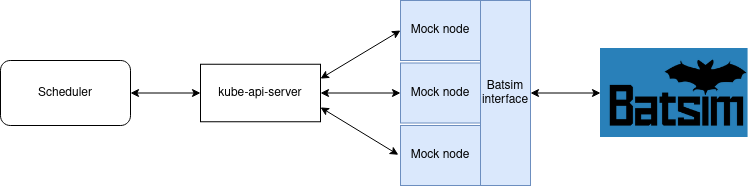
\includegraphics[width=\textwidth]{imgs/architecture-as-kubelets.png}
	\caption{Mocking the cluster itself.}
	\label{fig:mock_nodes}
\end{figure}

\subsubsection{Custom client-go}

Most Kubernetes schedulers rely on
client-go\footnote{https://github.com/kubernetes/client-go}, which is a Go
client for the api-server. It is a library implementing various tools to help
schedulers converse with the API. By altering this client and patching
schedulers so they use our client instead, we can make it exchange with Batsim
instead of the API. 

\begin{figure}[h]
	\centering
	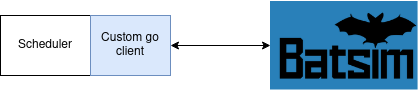
\includegraphics[scale=0.8]{imgs/custom-go-client.png}
	\caption{Custom Go client to redirect scheduler communications to Batsim}
	\label{fig:custom-go-client}
\end{figure}

Contrary to the kubelets, client-go is a user interface and therefore it is
documented, facilitating reverse engineering of its source code. Still, it
represents thousands of lines of code and altering it to our needs would not be
an easy feat.  The other drawback to this approach is that Batkube would only
support schedulers written in Go and making use of client-go, although this
should not be an issue as the only kubernetes scheduler we could find that does
not rely on client-go is a toy scheduler written in bash \cite{bash-scheduler}.

\subsubsection{Partial reimplementation of the API}

Re-implementing the API offers a middle ground between the low level and
undocumented solution of the mock nodes, and the higher level and technically
challenging solution of a client-go fork. Again, there are several options here.

A partial reimplementation of the API would save us the task of building a new
API from the ground up. However this would imply digging deep into the
api-server code in order to understand how the api is organized and what code
we would have to alter. In the end, it is easier to simply build a new API,
since there are tools to help us generate it from its specification.

\begin{figure}[h]
	\centering
	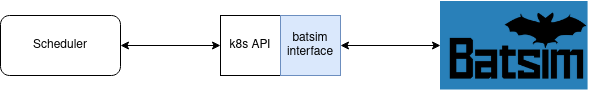
\includegraphics[scale=0.8]{imgs/partial-reimplem.png}
	\caption{Partial reimplementation of the api-server.}
	\label{fig:partial_reimp}
\end{figure}

\section{Time interception: the C library approach}

An attempt was first made to patch a custom C library, which is the lowest level
solution. Going for the low level solution would truly redirect all calls to
machine time which is something we can not guarantee with the second option, as
we explain in section \ref{sec:patch-scheds}. This approach proved challenging
due to circular dependency issues and was ultimately abandoned. We opted for
the second option which consist of modifying Go source code, which requires
some additional work to patch the schedulers but was actually easier to
implement.

\begin{figure}
	\centering
	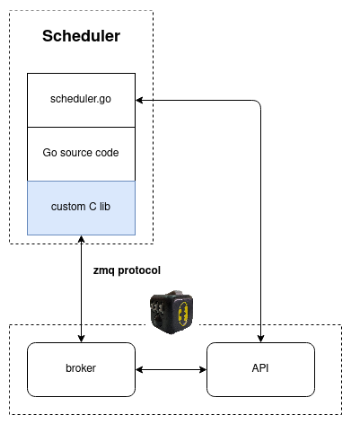
\includegraphics[scale=0.5]{imgs/time-hijack-C.png}
	\caption{Option A: patching the C library}
	\label{fig:patch-C}
\end{figure}


\backmatter
\printbibliography
\end{document}
